\documentclass[12pt,draftclsnofoot,onecolumn]{IEEEtran}

\renewcommand{\baselinestretch}{1.2}
\textwidth 7.2in
\oddsidemargin -0.3in

\ifodd 1
\newcommand{\rev}[1]{{\color{blue}#1}} %revise of the text
\else
\newcommand{\rev}[1]{#1}
\fi



\usepackage{booktabs}


\usepackage{bbm}
\usepackage{amssymb}

%\usepackage{algorithm}
\usepackage{algpseudocode}

\usepackage{amssymb,amsmath,color,graphicx}
\usepackage{verbatim}
\usepackage{amsmath}
\usepackage{times,graphicx, amsfonts}
\usepackage{multicol}
\usepackage{caption}
\usepackage{array}
\usepackage{mathrsfs}
\usepackage{marvosym}
\usepackage{bm}
\usepackage{mathrsfs}
\usepackage{setspace}
\usepackage{changepage}
\usepackage{float}
\usepackage{subcaption}
\usepackage{amsthm,amsbsy}
\usepackage{textcomp}
\usepackage{xcolor}
\usepackage{mathtools}
\usepackage[sort,compress]{cite}
\usepackage[bookmarks=true]{hyperref}
\usepackage[ruled,commentsnumbered,linesnumbered]{algorithm2e}

\def\BibTeX{{\rm B\kern-.05em{\sc i\kern-.025em b}\kern-.08em
		T\kern-.1667em\lower.7ex\hbox{E}\kern-.125emX}}

\DeclareMathOperator*{\minimize}{minimize}

\newtheorem{theorem}{Theorem}
\newtheorem*{remark}{Remark}

\newenvironment{my}[2]%
{\begin{list}{}%
{\setlength{\rightmargin}{#1}\setlength{\leftmargin}{#2}}%


 \item[]{}

} {\end{list}}




%%%%%%%%%%%%%%%%%%%%%%%%%%%%%%%%%%%%%%%%%%%%%%%%%%%%%%%%%%%%%%%%%%%
\begin{document}
%%%%%%%%%%%%%%%%%%%%%%%%%%%%%%%%%%%%%%%%%%%%%%%%%%%%%%%%%%%%%%%%%%%


\begin{abstract}
	In the realm of mobile edge computing (MEC), efficient computation task offloading plays a pivotal role in ensuring a seamless quality of experience (QoE) for users. Maintaining a high QoE is paramount in today's interconnected world, where users demand reliable services. This challenge stands as one of the most primary key factors contributing to handling dynamic and uncertain mobile environment. In this study, we delve into computation offloading in MEC systems, where strict task processing deadlines and energy constraints can adversely affect the system performance. We formulate the computation task offloading problem as a Markov decision process (MDP) to maximize the long-term QoE of each user individually. We propose a distributed QoE-oriented computation offloading (QECO) algorithm based on deep reinforcement learning (DRL) that empowers mobile devices to make their offloading decisions without requiring knowledge of decisions made by other devices. Through numerical studies, we evaluate the performance of QECO. Simulation results validate that QECO efficiently exploits the computational resources of edge nodes. Consequently, it can complete 14\% more tasks and reduce task delay and energy consumption by 9\% and 6\%, respectively. These together contribute to a significant improvement of at least 37\% in average QoE compared to an existing algorithm.
\end{abstract}

\begin{IEEEkeywords}
	Mobile edge computing, computation task offloading, quality of experience, deep reinforcement learning.
\end{IEEEkeywords}

\section{Introduction} 


Mobile edge computing (MEC) \cite{mao2017survey} has emerged as a promising technological solution to overcome the challenges faced by mobile devices (MDs) when performing high computational tasks, such as real-time data processing and artificial intelligence applications \cite{zhou2019edge} \cite{yousefpour2019all}. In spite of the MDs' technological advancements, their limited computing power and battery may lead to task drops, processing delays, and an overall poor user experience. By offloading intensive tasks to nearby edge nodes (ENs), MEC effectively empowers computation capability and reduces the delay and energy consumption. This improvement enhances the users' QoE, especially for time-sensitive computation tasks \cite{TNSE-QOE-24} \cite{ shah2018hierarchical}. 

Efficient task offloading in MEC is a complex optimization challenge due to the dynamic nature of the network and the variety of MDs and servers involved \cite{jiang2019toward} \cite{TNSE-WU-24}. In particular, determining the optimal offloading strategy, scheduling the tasks, and selecting the most suitable EN for task offloading are the main challenges that demand careful consideration. Furthermore, the uncertain requirements and sensitive latency properties of computation tasks pose nontrivial challenges that can significantly impact the computation offloading performance in MEC systems with limited resources.

\textcolor{blue}{To cope with the dynamic nature of the network, recent research has proposed several task offloading algorithms using machine learning methods. In particular, reinforcement learning (RL) hold promises to determine optimal decision-making policies by capturing the dynamics of environments and learning strategies for accomplishing long-term objectives \cite{arulkumaran2017deep}. RL can effectively tackle the challenges of MEC arising from the ever-changing nature of networks, MDs, and servers' heterogeneity. This ultimately improves the MD users' QoE. We explore state-of-the-art RL-based techniques characteristic to discuss how they address task offloading problems in MEC. To minimize energy consumption, Munir \textit{et al.} \cite{munir2021multi} developed a semi-distributed approach using a multi-agent RL (MARL) framework for self-powered MEC. Gong \textit{et al.} in \cite{gong2022edge} proposed a DRL-based network structure in the industrial IoT (IIoT) systems to jointly optimize task offloading and resource allocation to achieve lower energy consumption and decreased task delay. To investigate privacy aware computation offloading problem, Wu \textit{et al.} in \cite{wu2024combining} proposed a deep Q-network (DQN)-based method. They transform the problem on MDP to optimize computation rate and energy consumption in a queuing-based IIoT network. Sun \textit{et al.} in \cite{sun2024hierarchical} explored both computation offloading and service caching problems in MEC. They formulated an optimization problem that aims to minimize the long-term average service delay. They then proposed a hierarchical DRL framework, which effectively handles both problems under heterogeneous resources.}









%Researchers have recently proposed several task offloading algorithms to tackle the aforementioned issues. Mao \textit{et al.} in \cite{mao2016dynamic} introduced a computation offloading algorithm for MEC systems. This scheme aims to reduce the MD's energy consumption while meeting the computation delay constraints. In \cite{zhang2016energy}, Zhang \textit{et al.} proposed an offloading scheme for MEC in heterogeneous cellular networks, taking into account the energy-constrained MEC scenario and the heterogeneity of MDs when optimizing the offloading decisions. Bi \textit{et al.} in \cite{bi2018computation} proposed an algorithm to optimize decision-making about computation offloading and power transferring in a wireless-powered MEC. Ning \textit{et al.} in \cite{ning2018cooperative} introduced a heuristic algorithm designed to enhance the efficiency of the partial computation offloading model. The works in \cite{mao2016dynamic}-\cite{ning2018cooperative} primarily focus on quasi-static systems and are not well-suited for dynamic systems and time-varying conditions. 

%The uncertain requirements and sensitive latency properties of computation tasks in MEC systems with limited resources pose nontrivial challenges that can significantly impact the computation offloading performance. In \cite{jovsilo2019wireless}, Josilo \textit{et al.} proposed a distributed algorithm based on a Stackelberg game. Lee \textit{et al.} in \cite{lee2019online} designed an algorithm based on online optimization techniques to minimize the maximum delay of the tasks in a hybrid edge-cloud network. Yang \textit{et al.} in \cite{yang2018distributed} explored an overhead minimization problem, aiming to jointly optimize delay and energy consumption in MEC. They proposed a distributed offloading algorithm to mitigate the wireless channel competition among MDs. The works \cite{jovsilo2019wireless}-\cite{yang2018distributed} considered delay-tolerant tasks, which may have a limited applicability due to the real-time processing demand of high computational tasks. Compared to these works, we explore a more realistic MEC scenario involving delay-sensitive tasks with processing deadlines, which poses a more complex challenge.

%presents a more challenging problem. The impact of processing deadlines on the dynamic workload at the ENs influences the delay experienced by the offloaded tasks. 


%In \cite{mao2016dynamic,zhang2016energy,bi2018computation,ning2018cooperative}, the processing capacity assigned to each MD by an EN remained unaffected by the number of offloaded tasks, resulting in a heavy load on the EN when a significant number of MDs offload their tasks to it. This heavy load can cause significant processing delays and even lead to missed deadlines and dropped tasks. To mitigate this issue, some existing works have proposed task offloading algorithms that consider the workloads at the ENs. In \cite{chen2018task}, Chen \textit{et al.} proposed an algorithm for task offloading in a software-defined ultra-dense network. The goal of this algorithm is to minimize task delay by formulating the task offloading scheme as a mixed integer non-linear program problem. Shah-Mansouri \textit{et al.} in \cite{shah2018hierarchical} proposed a QoE maximization slotwork for offloading decisions based on computation energy and delay reduction. They formulated a potential game to model competition among IoT users and achieved a close-to-optimal social cost.


\subsection{Related Work}
%\textcolor{black}{We explore state-of-the-art techniques characteristic to discuss how they address task offloading problems in scenarios that need to process massive data with limited devices in MEC, such as the Internet of Things (IoT), Internet of Vehicles (IoV), and Industrial IoT (IIoT)  environment. 
	
	
	
	%Internet of Things (IoT) \cite{dai2020edge}, \cite{liao2023online}, \cite{Bolourian-WCL24}, 
	%Internet of Vehicles (IoV) \cite{Bolourian-WCL24}, 
	%and Industrial IoT (IIoT)  environment \cite{gong2022edge}, \cite{wu2023multi}, \cite{wu2024combining}
	
	
	%\subsubsection{DRL-Based Task Offloading Optimization in MEC}
	
	\textcolor{blue}{
		In recent years, edge computing has become a popular method for scenarios that need to process massive data with weak devices, such as IoTs \cite{zhang2023multi}, Internet of Vehicles (IoVs) \cite{lin2022multi}, \cite{wei2023many}, and Industrial IoT (IIoT) \cite{yuan2023adaptive} environment. To take advantage of RL methods for online computation offloading in MEC, Huang \textit{et al.} in \cite{huang2019deep}, focused on a wireless-powered MEC. They proposed a DRL-based approach, capable of attaining near-optimal decisions. This is achieved by selectively considering a compact subset of candidate actions in each iteration. Liu \textit{et al.} in \cite{liu2021learn} investigated a two-timescale computing offloading and resource allocation problem and proposed a resource coordination algorithm based on multi-agent DRL (MADRL), which can generate interactive information along with resource decisions. Zhou \textit{et al.} in \cite{zhou2021deep} used an MDP to model the interactions of the environment. They proposed a Q-learning approach to achieve optimal resource allocation strategies and computation offloading. Liao \textit{et al.} in \cite{liao2023online} introduced a double DRL algorithm for performing online computation offloading in MEC. This algorithm optimizes transmission power and scheduling of CPU frequency when minimizing both task computation delay and energy consumption. }
	
	\textcolor{blue}{
		In these researches authors investigated simple MEC networks and explored computation offloading problems, mainly focused on delay-tolerant tasks or single MEC network model, and did not take into account the challenges of dynamic network environment with the variety of MDs and servers involved. In actual scenarios, an MEC system can provide delay-constrained services for serval MDs and ENs at the same time, while the works \cite{huang2019deep}, \cite{liu2021learn} not consider delay-sensitive tasks for network model and \cite{zhou2021deep}, \cite{liao2023online} just considered the situation of a single server or user in the MEC system.}
	
	\textcolor{blue}{  
		In fact, the state of MD's computing and transmission power, arrived task's requirement, the energy state of MDs, and workloads at ENs all change dynamically with time in actual systems, thus a more realistic MEC scenario is needed. Besides the works \cite{huang2019deep}--\cite{liao2023online}, Wu \textit{et al.} in \cite{wu2023computation} introduced a stochastic game-based resource allocation in the SDN-based MEC network. They used an MDP and proposed a MARL method to minimize both energy consumption and processing delay. Dai \textit{et al.} in \cite{dai2020edge} introduced the integration of action refinement into DRL and designed an algorithm to concurrently optimize resource allocation and computation offloading. To optimize privacy protection and quality of service, authors in \cite{wu2024privacy} investigated the joint computation offloading and power allocation problems for the IIoT network. They modeled the problem as an MDP and proposed a multi-agent DDQN-based algorithm.
		In \cite{zhao2019deep}, Zhao \textit{et al.} proposed a computation offloading algorithm based on DRL, which addresses the competition for wireless channels to optimize long-term downlink utility. In this approach, each MD requires quality-of-service information from other MDs.}
	
	
	
	
	
	%In these researchs authours mostly investigated MEC networks and explored computation offloading problem, but in some works such as \cite{zhou2021deep} \cite{liao2023online} have mainly focused on single MEC network model, and has not taken into account the challenges of dynamic network environment with multiple ENs. In fact, the channel quality, requested task, and energy state on an MDs all change dynamically with time in an actual MEC scenario, thus a more realistic MEC scenario is needed, involving delay-sensitive tasks with processing deadlines in multiple MDs and ENs, which poses a more intricate challenge.
	
	
	\textcolor{blue}{
		While studies like \cite{wu2023computation}--\cite{zhao2019deep} explored task offloading problems in a more advanced scenario and proposed some DRL-based algorithms, MEC systems often encounter challenges related to managing time-varying resource requests from heterogeneous devices, imposing significant challenges in resource accessibility and overall system performance. To address this issue, the authors applied queuing theory to model MEC systems more accurately, reflecting real-world scenarios. 
		%\subsubsection{Queuing Theory for Computation Offloading}
		In \cite{Bolourian-WCL24}, the authors proposed an offloading algorithm using deep Q-learning for wireless-powered IoT devices in MEC systems. This algorithm aims to minimize the task drop rate while the devices solely rely on harvested energy for operation. Tang \textit{et al.} in \cite{9253665} investigated the task offloading problem for indivisible and deadline-constrained computational tasks in MEC systems. The authors proposed a distributed DRL-based offloading algorithm designed to handle uncertain workload dynamics at the ENs. 
		In \cite{huang2021deadline}, Huang \textit{et al.} proposed a DRL-based method based on a partially observable MDP (POMDP), which guarantees the deadlines of real-time tasks while minimizing the total energy consumption of MDs. This algorithm effectively tackles the challenges of dynamic resource allocation in large-scale heterogeneous networks. To optimize delay and energy consumption in an MEC-based IIoT system, Wu \textit{et al.} in \cite{wu2023multi} proposed a multi-agent DQN-based method based on POMDP to address computation offloading problem. In \cite{gao2022large}, Gao \textit{et al.} introduced an attention-based multi-agent algorithm designed for decentralized computation offloading.}
	

%	\begin{table*}[htbp]\textcolor{blue}{
%		\renewcommand{\arraystretch}{0.6}
%		\captionsetup{name=TABLE}
%		\caption{Comparison of Related Works Characteristic\vspace{4mm}}
%		\scalebox{0.7}{%
%			\begin{tabular}{ lp{3.4cm}p{4.5cm}p{5.2cm}p{1.7cm}p{3cm}p{4.6cm}l} 
%				\toprule
%				\textbf{Paper} & \textbf{Scenario} &  \textbf{Problem} &  \textbf{Objective} &  \textbf{Model} & \textbf{Method} &  \textbf{Drawbacks}  \\ \midrule
%				\cite{liao2023online} & Queuing-based MEC & Online computation offloading & Minimize computation delay and energy consumption & MDP & DDQN & Only for a singel MEC system model  \\\midrule
%				\cite{zhou2021deep} & heterogeneous MEC & Resource allocation and computation offloading & Minimize energy consumption of the entire system & MDP & DDQN & Only for a singel MEC system model \\\midrule				
%				\cite{huang2019deep} & Wireless-powered MEC & Computation offloading and resource allocations & Maximize computation rate & MIP & DQN & Not consider delay-sensitive tasks \\\midrule
%				\cite{wu2024privacy} & MEC-based IIoT  & Joint power allocation and computation offloading  & Optimization of privacy protection and quality of service. & MDP & Multi-agent DDPG & Not take user's deman into consideration \\\midrule
%				\cite{zhao2019deep} & MEC & User association and resource allocation & Optimize downlink utility & MDP & Multi-agent D3QN & Not consider system delay and energy consumtion \\\midrule
%				\cite{sun2024hierarchical} & MEC & Computation offloading and service caching & Minimize average service delay & MDP & hierarchical DRL & Not consider system energy consumtion \\\midrule
%				\cite{wu2023computation} & SDN-based MEC & Stochastic game-based resource allocation & Minimize energy consumption and processing delay & MDP & MARL & Not consider tasks with maximum delay tolerance\\\midrule
%				\cite{dai2020edge} & MEC & Resource allocation and computation offloading & Minimize energy consumption & MDP & DDPG & Not take user's deman into consideration \\\midrule
%				\cite{liu2021learn} & MEC & Resource allocation and computation offloading & Minimize execution cost & POMDP & MADRL &  Not consider delay-sensitive tasks \\\midrule
%				\cite{gong2022edge} & MEC-based IIoT & Resource allocation and computation offloading & Minimize task computation delay and energy consumption & MDP & DRL & Not take user's deman into consideration\\\midrule
%				\cite{gao2022large} & Queuing-based heterogeneous MEC & Decentralized computation offloading & Optimize system cost and completion rates & MDP & Multi-agent DDPG & Not take user's deman into consideration \\\midrule
%				\cite{9253665} &  Queuing-based MEC &  Computation offloading & Minimize drop rate and computation delay. & MDP & D3QN + LSTM & Not consider system energy consumtion\\\midrule
%				\cite{wu2024combining} & Queuing-based IIoT MEC & Privacy aware computation offloading & Optimization of computation rate and energy consumption & MDP & DDPG  & Not take user's deman into consideration \\\midrule
%				\cite{wu2023multi} & Queuing-based IIoT MEC & Computation offloading & Optimize delay and energy consumption & POMDP & Multi-agent DQN&  Not consider tasks with maximum delay tolerance \\\midrule
%				\cite{huang2021deadline} & Queuing-based MEC & Computation offloading & Optimize drop rate and energy consumption & POMDP & DDPG & Not consider computation delay \\ \midrule
%				\cite{Bolourian-WCL24} & Queuing-based MEC with EHs& Energy harvesting  computation offloading & Minimize drop rate and energy consumption. & MDP  & DQN & Not consider computation delay  \\\midrule
%				QECO &  Queuing-based MEC &  Computation offloading & Maximize the QoE of each MD individually &MDP & D3QN + LSTM & \\
%				\toprule
%		\end{tabular}}
%		\label{table1}}
%\end{table*}
	
	
	
	\subsection{Motivation and Contributions}
	
	Although DRL-based methods have demonstrated their effectiveness in handling network dynamics, task offloading still encounters several challenges that require further attention.  \textcolor{blue}{As shown in Table~\ref{table1}, current research primarily focuses on minimizing energy consumption \cite{tang2022uav}, reducing processing delays \cite{guo2022energy}, \cite{seo2022differential}, maximizing computation rates~\cite{huang2019deep}, or optimizing a weighted balance among performance factors \cite{li2022joint}. However, QoE is a time-varying performance measure that reflects user satisfaction and is not affected only by delay, as considered in \cite{sun2024hierarchical}, \cite{9253665} but also by energy consumption \cite{Bolourian-WCL24}, \cite{huang2021deadline}. A more comprehensive approach is required to address the dynamic requirements of individual users in real-time scenarios with multiple MDs and ENs. 
		While some existing works such as \cite{liao2023online}, \cite{wu2024privacy}, \cite{dai2020edge}, \cite{gao2022large}, \cite{li2022joint} have investigated the trade-off between delay and energy consumption, they fail to address the user demands and fulfill QoE requirements properly.} In contrast to the aforementioned works, we propose a DRL-based distributed algorithm that provides users with an appropriate balance among QoE factors based on their demands. %We also explore a more realistic MEC scenario involving delay-sensitive tasks with processing deadlines, posing a more intricate challenge.
	
	



In this study, we delve into the computation task offloading problem in MEC systems, where strict task processing deadlines and energy constraints can adversely affect the system performance. We propose a distributed QoE-oriented computation offloading (QECO) algorithm that leverages DRL to efficiently handle task offloading in uncertain loads at ENs. This algorithm empowers MDs to make offloading decisions utilizing only locally observed information, such as task size, queue details, battery status, and historical workloads at the ENs. By adopting the appropriate policy based on each MD’s specific requirements at any given time, the QECO algorithm significantly improves the QoE for individual users.



%Inspired by existing studies, we delve into the challenge of computation task offloading in MEC systems, where the presence of strict task processing deadlines and energy constraints can adversely affect system performance and cause task delays. We proposes a decentralized offloading algorithm that empowers MDs to make intelligent decisions about offloading. The primary focus of our research is on the partial STO problem, where tasks can be fragmented into smaller sub-tasks, and the workloads at ENs can fluctuate dynamically and unpredictably. Our primary objective is to enhance the users' QoE individually. To define the problem, we have formulated the energy constraint MEC system as a Markov decision process (MDP) problem. To solve the MDP problems, Reinforcement Learning provides a range of solution methods such as dynamic programming, Monte Carlo methods, and temporal-difference learning. To deal with the Curse of Dimensions, modern Reinforcement Learning methods apply nonlinear function approximation, such as deep Q-network (DQN), to solve the problem with large state and action spaces. In our proposed approach, we leverage deep Q-learning \cite{mnih2015human}, a model-free DRL technique that enables agents to make informed decisions based on local observations without explicit knowledge of the system's dynamics and modeling. Compared to other researches, our approach provides a more realistic MEC scenario and a promising solution to the challenging problem of task offloading with strict deadline constraints. The proposed algorithm, by only utilizing locally observed information, allows each MD to determine the offloading decision in a decentralized manner. 

Our main contributions are summarized as follows:

\begin{itemize}
	\item \textit{Task Offloading Problem in the MEC System:} We formulate the task offloading problem as an MDP for time-sensitive tasks. This approach takes into account the dynamic nature of workloads at the ENs and concentrates on providing high performance in the MEC system while maximizing the long-term QoE.
	
	\item \textit{DRL-based Offloading Algorithm:} To address the problem of long-term QoE maximization, we focus on task completion, task delay, and energy consumption to quantify the MDs' QoE. We propose QECO algorithm based on DRL that empowers each MD to make offloading decisions independently, without prior knowledge of the other MDs' tasks and offloading models. With a focus on the MD's battery level, our approach leverages deep Q-network (DQN) \cite{mnih2015human} and long short-term memory (LSTM) \cite{hochreiter1997long} to prioritize and strike an appropriate balance between QoE factors. We also analyze the training convergence and complexity of the proposed algorithm.
	
	\item \textit{Performance Evaluation:} We conduct comprehensive experiments to evaluate the QECO's performance as well as its training convergence under different computation workloads. The results demonstrate that our algorithm quickly converges and effectively utilizes the processing capabilities of MDs and ENs, resulting in substantial improvement of at least 37\% in average QoE. This advantage is achieved through a 14\% increase in the number of completed tasks, along with 9\% and 6\% reductions in task delay and energy consumption, respectively, when compared to the potential game-based offloading algorithm (PGOA) \cite{yang2018distributed} and several benchmark methods.
	
	
	
\end{itemize}

The structure of this paper is as follows. Section~\ref{section:II} presents the system model, followed by the problem formulation in Section ~\ref{section:III}. In Section~\ref{section:IV}, we present the algorithm, while Section~\ref{section:V} provides an evaluation of its performance. Finally, we conclude in Section~\ref{section:VI}.


\section{System Model} 
\label{section:II}
\label{sec:latexhints}
% Required for proper example rendering in the compiled PDF
\newcount\LTGbeginlineexample
\newcount\LTGendlineexample
\newenvironment{ltgexample}%
{\LTGbeginlineexample=\numexpr\inputlineno+1\relax}%
{\LTGendlineexample=\numexpr\inputlineno-1\relax%
	%
	\tcbinputlisting{%
		listing only,
		listing file=\currfilepath,
		colback=green!5!white,
		colslot=green!25,
		coltitle=black!90,
		coltext=black!90,
		left=8mm,
		title=Corresponding \LaTeX{} code of \texttt{\currfilepath},
		listing options={%
			slot=none,
			language={[LaTeX]TeX},
			escapeinside={},
			firstline=\the\LTGbeginlineexample,
			lastline=\the\LTGendlineexample,
			firstnumber=\the\LTGbeginlineexample,
			basewidth=.5em,
			aboveskip=0mm,
			belowskip=0mm,
			numbers=left,
			xleftmargin=0mm,
			numberstyle=\tiny,
			numbersep=8pt%
		}
	}
}%
We investigate a MEC system consisting of a set of MDs denoted by $\mathcal{I} = \{1, 2, ..., I\}$, along with a set of ENs denoted by $\mathcal{J} = \{1, 2, ..., J\}$, where $I$ and $J$ represent the number of MDs and ENs, respectively. We regard time as a specific episode containing a series of $T$ time slots denoted by $\mathcal{T} = \{1, 2, \ldots, T\}$, each representing a duration of $\tau$ seconds. As shown in Fig.~\ref{fig1}, we consider two separate queues for each MD to organize tasks for local processing or dispatching to ENs, operating in a first-in-first-out (FIFO) manner. The MD's scheduler is responsible for assigning newly arrived tasks to each of the queues at the beginning of the time slot. On the other hand, we assume that each EN $j \in \mathcal{J}$ consists of $I$ FIFO queues, where each queue corresponds to an MD $i \in \mathcal{I}$. When each task arrives at an EN, it is enqueued in the corresponding MD's queue. %We assume that if a task is completed in a certain time slot, the next task in the queue will start its operation at the beginning of the next time slot.

\begin{figure}
	\captionsetup{name=Fig.}
	\centering
	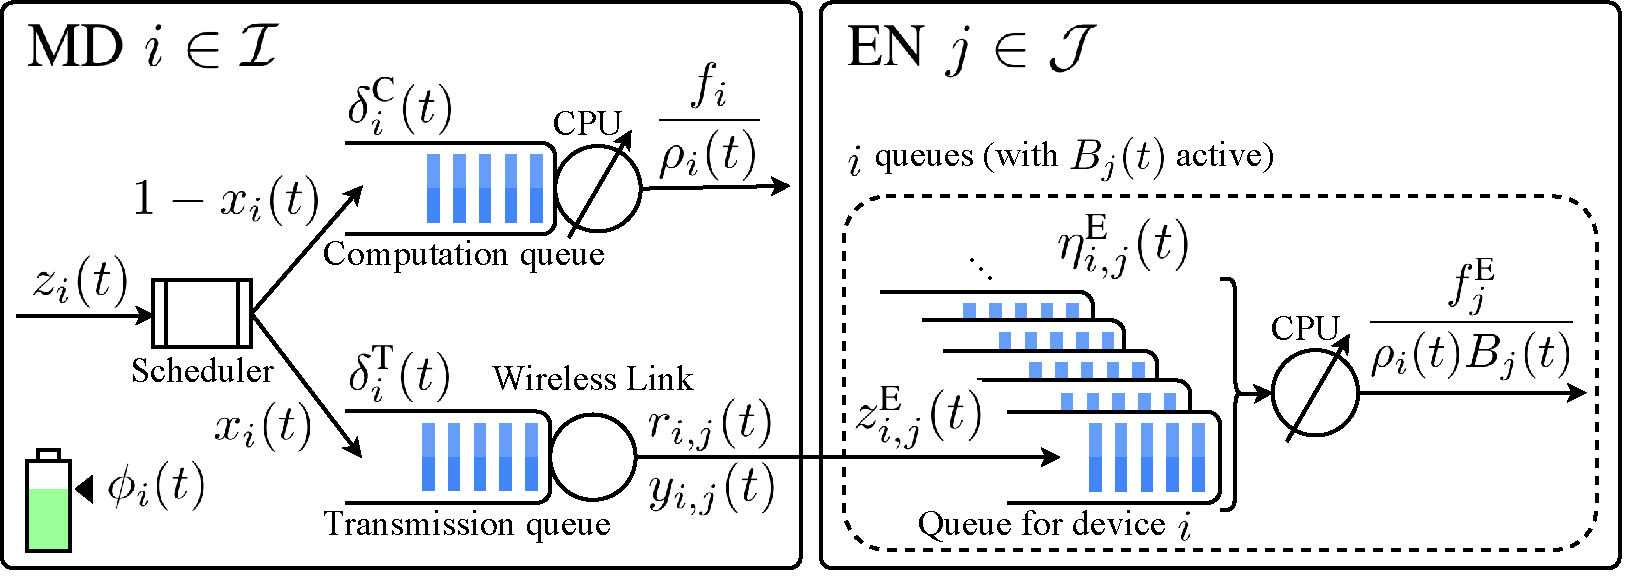
\includegraphics[width=.7\linewidth]{ queue}
	\vspace*{-1mm}
	\caption{An illustration of MD $i \in \mathcal{I}$ and EN $j \in \mathcal{J}$ in the MEC system.}
	\vspace*{-3mm}
	\label{fig1}
\end{figure}

We define $z_i(t)$ as the index assigned to the computation task arriving at MD $i \in \mathcal{I}$ in time slot $t \in \mathcal{T}$. Let $\lambda_i(t)$ denote the size of this task in bits. The size of task $z_i(t)$ is selected from a discrete set $\Lambda = \{\lambda_1, \lambda_2, \ldots, \lambda_{\theta}\}$, where $\theta$ represents the number of these values. Hence, $\lambda_i(t) \in \Lambda \cup \{0\}$ to consider the case that no task has arrived. We also denote the task's processing density as $\rho_i(t)$ that indicates the number of CPU cycles required to complete the execution of a unit of the task. Furthermore, we denote the deadline of this task by $\Delta_i(t)$ which is the number of time slots that the task must be completed to avoid being dropped.
%At the beginning of time slot $t \in \mathcal{T}$, if MD $i \in \mathcal{I}$ has a newly arrived task, we define $z_i(t)$ as the unique index assigned to that task. Let $\lambda_i(t)$ be the number of newly arrived bits at the beginning of time slot $t \in \mathcal{T}$. If a new task $z_i(t)$ exists at the start of time slot $t$, then $\lambda_i(t)$ is equal to the size of task $z_i(t)$. Otherwise, $\lambda_i(t) = 0$. We consider $\rho_i(t)$ to represent the processing density of task $z_i(t)$, indicating the number of CPU cycles required to process a unit of the task.

We define two binary variables, $x_i(t)$ and $y_{i,j}(t)$ for $i \in \mathcal{I}$ and $j \in \mathcal{J}$ to determine the offloading decision and offloading target, respectively. Specifically, $x_i(t)$ indicates whether task $z_i(t)$ is assigned to the computation queue ($x_i(t) = 0$) or to the transmission queue ($x_i(t) = 1$), and $y_{i,j}(t)$ indicates whether task $z_i(t)$ is offloaded to EN $j \in \mathcal{J}$. If the task is dispatched to EN $j$, we set $y_{i,j}(t) = 1$; otherwise, $y_{i,j}(t) = 0$.





\subsection{Communication Model}
We consider that the tasks in the transmission queue are dispatched to the appropriate ENs via the MD wireless interface. We denote the transmission rate of MD $i$'s interface when communicating with EN $j \in \mathcal{J}$ in time $t$ as $r_{i,j}(t)$. In time slot $t \in \mathcal{T}$, if task $z_i(t)$ is assigned to the transmission queue for computation offloading, we define $l_i^{\text{T}}(t) \in \mathcal{T}$ to represent the time slot when the task is either dispatched to the EN or dropped. We also define $\delta_i^{\text{T}}(t)$ as the number of time slots that task $z_i(t)$ should wait in the queue before transmission. It should be noted that MD $i$ computes the value of $\delta_i^{\text{T}}(t)$ before making a decision. The value of $\delta_i^{\text{T}}(t)$ is computed as follows:
\begin{alignat}{1}
	\delta_i^{\text{T}}(t) =\textcolor{white}{i} \left[ \textcolor{white}{i}\max\limits_{t^{'}\textcolor{white}{i} \in \textcolor{white}{i} \{0,1,\ldots,t-1\}} l_i^{\text{T}}\textcolor{white}{i}(t^{'})-t+1\textcolor{white}{i}\right]^+\textcolor{white}{i},
	\label{1}  
\end{alignat}
where $[\cdot]^+ =$ max$(0, \cdot)$ and $l_i^{\text{T}}(0)=0$ for the simplicity of presentation. Note that the value of $\delta_i^{\text{T}}(t)$ only depends on $l_i^{\text{T}}(t)$ for $t' < t$. If MD $i \in \mathcal{I}$ schedules task $z_i(t)$ for dispatching in time slot $t \in \mathcal{T}$, then it will either be dispatched or dropped in time slot $l_i^{\text{T}}(t)$, which is
\begin{alignat}{1}
	l_i^{\text{T}}(t) = \min \Big\{t + \delta_i^{\text{T}}(t) + \lceil{D_i^{\text{T}}(t)}\rceil - 1, t + \Delta_i(t) - 1\Big\},
	\label{2}  
\end{alignat}
where $D_i^{\text{T}}(t)$ refers to the number of time slots required for the transmission of task $z_i(t)$ from MD $i \in \mathcal{I}$ to EN $j \in \mathcal{J}$. We have
\begin{alignat}{1}
	D_i^{\text{T}}(t) =  \sum_{\mathcal{J}} y_{i,j}(t) {\lambda_i(t) \over r_{i,j}(t)\tau}.
	\label{3}  
\end{alignat}
Let $E_i^{\text{T}}(t)$ denote the energy consumption of the transmission from MD $i \in \mathcal{I}$ to EN $j \in \mathcal{J}$. We have
\begin{alignat}{1}
	E_i^{\text{T}}(t) = D_i^{\text{T}}(t)p_i^{\text{T}}(t)\tau,
	\label{4}  
\end{alignat}
where $p_i^{\text{T}}(t)$ represents the power consumption of the communication link of MD $i \in \mathcal{I}$ in time slot $t$.
\subsection{Computation Model}
The computation tasks can be executed either locally on the MD or on the EN. In this subsection, we provide a detailed explanation of these two cases.
\subsubsection{Local Execution}
We model the local execution by a queuing system consisting the computation queue and the MD processor. Let $f_i$ denote the MD $i$'s processing power (in cycle per second). When task $z_i(t)$ is assigned to the computation queue at the beginning of time slot $t \in \mathcal{T}$, we define $l_i^{\text{C}}(t) \in \mathcal{T}$ as the time slot during which task $z_i(t)$ will either be processed or dropped. If the computation queue is empty, $l_i^{\text{C}}(t) = 0$. Let $\delta_i^{\text{C}}(t)$ denote the number of remaining time slots before processing task $z_i(t)$ in the computation queue. We have:
\begin{alignat}{1}
	\delta_i^{\text{C}}(t) = \left[ \max \limits_{t' \in \{0,1,\ldots,t-1\}} l_i^{\text{C}}(t')-t+1 \right]^+.
	\label{5}  
\end{alignat}
%In the above relation, the operator $[z]^+ = \max{0, z}$ is defined, and the variable $l_i^{\text{C}}(0) = 0$. Specifically, the expression $\max_{t' \in {0,1,2,\ldots,t-1}} l_i^{\text{C}}(t')$ determines the time slot until which all tasks placed in the local computation queue have been completed before time slot $t$. Therefore, $\delta_i^{\text{C}}(t)$ represents the number of time slots that task $z_i(t)$ needs to wait for processing. For example, suppose task $z_i(1)$ is in the computation queue, and its processing will be completed in time slot 5. Hence, $l_i^{\text{C}}(1) = 5$, meaning that the task should remain in the queue for $\Delta^{comp}(3) = [\max{5,0}-3+1]^+ = 3$ time slots until the process is finished.
In the equation above, the term $\max_{t' \in \{0, 1, \ldots, t-1\}} l_i^{\text{C}}(t')$ denotes the time slot at which each existing task in the computation queue, which arrived before time slot $t$, is either processed or dropped. Consequently, $\delta_i^{\text{C}}(t)$ denotes the number of time slots that task $z_i(t)$ should wait before being processed. We denote the time slot in which task $z_i(t)$ will be completely processed by $l_i^{\text{C}}(t)$ if it is assigned to the computation queue for local processing in time slot $t$. We have
\begin{alignat}{1}
	l_i^{\text{C}}(t) = \min \Big\{t + \delta_i^{\text{C}}(t) + \lceil D_i^{\text{C}}(t) \rceil - 1, t + \Delta_i(t) - 1\Big\}.
	\label{6}  
\end{alignat}
The task $z_i(t)$ will be immediately dropped if its processing is not completed by the end of the time slot $t + \Delta_i(t) - 1$. In addition, we introduce $D_i^{\text{C}}(t)$ as the number of time slots required to complete the processing of task $z_i(t)$ on MD $i \in \mathcal{I}$. It is given by:
\begin{alignat}{1}
	D_i^{\text{C}}(t) = { \lambda_i(t)  \over  f_i  \tau /  \rho_i(t)}.
	\label{7}  
\end{alignat}



%In particular, the processing of task $z_i(t)$ will commence at time $t + \delta_i^{\text{C}}(t)$. Therefore, the first component of the minimum operator is equal to the duration of time in which task $z_i(t)$ is completed without exceeding its deadline, denoted by $\delta_i^{\text{C}}(t)$. The second component refers to the duration of time in which task $z_i(t)$ becomes expired and discarded. As a result, $l_i^{\text{C}}(t)$ represents the time slot in which task $z_i(t)$ will be completed.
To compute the MD's energy consumption in the time slot $t \in \mathcal{T}$, we define $E_i^{\text{L}}(t)$ as:
\begin{alignat}{1}
	E_i^{\text{L}}(t) =  D_i^{\text{C}}(t) p_i^{\text{C}}  \tau, %=  { \lambda_i(t) \rho_i(t)  \over  f_i} p_i^{\text{C}},
	\label{8}  
\end{alignat}
where $p_i^{\text{C}} = 10^{-27}(f_i)^3$ represents the energy consumption of MD $i$'s CPU frequency \cite{mao2016dynamic}.
\subsubsection{Edge Execution}
We model the edge execution by the queues associated with MDs deployed at ENs. If computation task $z_i(t')$ is dispatched to EN $j$ in time $t' < t$, we let $z_{i,j}^{\text{E}}(t)$ and $\lambda_{i,j}^{\text{E}}(t)$ (in bits) denote the unique index of the task and the size of the task in the $i^{\text{th}}$ queue at EN $j$. We define $\eta_{i,j}^{\text{E}}(t)$ (in bits) as the length of this queue at the end of time slot $t \in \mathcal{T}$. We refer to a queue as an active queue in a certain time slot if it is not empty. That being said, if at least one task is already in the queue from previous time slots or there is a task arriving at the queue, that queue is active. We define $\mathcal{B}_j(t)$ to denote the set of active queues at EN $j$ in time slot $t$.
\begin{alignat}{1}
	\mathcal{B}_j(t) = \textcolor{white}{i}\Big\{i \textcolor{white}{i}\big| i \in \mathcal{I}, \lambda_{i,j}^{\text{E}}(t)>0\,\, \textcolor{white}{i}\text{or}\textcolor{white}{i} \,\, \eta_{i,j}^{\text{E}}(t-1)>0\textcolor{white}{i}\Big\}.\textcolor{white}{i}
	\label{9}  
\end{alignat}
We introduce $b_j(t) \triangleq |\mathcal{B}_j(t)|$ that represents the number of active queues in EN $j \in \mathcal{J}$ in time slot $t \in \mathcal{T}$. In each time slot $t \in \mathcal{T}$, the EN's processing power is divided among its active queues using a generalized processor sharing method~\cite{parekh1993generalized}. Let variable $f_j^{\text{E}}$ (in cycles per second) represent the computational capacity of EN $j$. Therefore, EN $j$ can allocate computational capacity of $f_j^{\text{E}}/(\rho_i(t) b_j(t))$ to each MD $i \in \mathcal{B}_j(t)$ during time slot $t$. To calculate the length of the computation queue for MD $i \in \mathcal{I}$ in EN $j \in \mathcal{J}$, we define $\omega_{i,j}(t)$ (in bits) to represent the number of bits from dropped tasks in that queue at the end of time slot $t \in \mathcal{T}$. The backlog of the queue, referred to as $\eta_{i,j}^{\text{E}}(t)$ is given by:
\begin{alignat}{1}
	\eta_{i,j}^{\text{E}}(t)\hspace{-0.8mm}=\hspace{-1mm}\left[\eta_{i,j}^{\text{E}}(t-1)\hspace{-0.6mm}+\hspace{-0.7mm}\lambda_{i,j}^{\text{E}}(t)\hspace{-0.7mm}-\hspace{-0.7mm}{f_j^{\text{E}}\tau\over \rho_i(t)b_j(t)} -\omega_{i,j}(t)\right]^+\hspace{-1mm}.
	\label{10}  
\end{alignat}
We also define $l_{i,j}^{\text{E}}(t) \in \mathcal{T}$ as the time slot during which the offloaded task $z_{i,j}^{\text{\text{E}}}(t)$ is either processed or dropped by EN $j$. Given the uncertain workload ahead at EN $j$, neither MD $i$ nor EN $j$ has information about $l_{i,j}^{\text{E}}(t)$ until the corresponding task $z_{i,j}^{\text{E}}(t)$ is either processed or dropped. Let $\hat{l}_{i,j}^{\text{E}}(t)$ represent the time slot at which the execution of task $z_{i,j}^{\text{E}}(t)$ starts. In mathematical terms, for $i \in \mathcal{I}$, $j \in \mathcal{J}$, and $t \in \mathcal{T}$, we have:
\begin{alignat}{1}
	\hat{l}_{i,j}^{\text{E}}(t) = \max \{t, \max \limits_{t^{'} \in \{0,1,\ldots,t-1\}} l_{i,j}^{\text{E}}(t^{'})+1\},
	\label{11}  
\end{alignat}
where $l_{i,j}^{\text{E}}(0) = 0$. Indeed, the initial processing time slot of task $z_{i,j}^{\text{E}}(t)$ at EN should not precede the time slot when the task was enqueued or when the previously arrived tasks were processed or dropped. Therefore, $l_{i,j}^{\text{E}}(t)$ is the time slot that satisfies the following constraints. %For $i \in \mathcal{I}$, $j \in \mathcal{J}$, and $t \in \mathcal{T}$,
\begin{alignat}{1}
	\sum_{t^{'}=\hat{l}_{i,j}^{\text{E}}(t)}^{l_{i,j}^{\text{E}}(t)}{f_j^{\text{E}}\tau \over \rho_i(t)b_j(t^{'})}\mathbbm{1}(i \in \mathcal{B}_j(t^{'}))  \geq   \lambda_{i,j}^{\text{E}}(t),
	\label{12}  \\
	\sum_{t^{'}=\hat{l}_{i,j}^{\text{E}}(t)}^{l_{i,j}^{\text{E}}(t)-1}{f_j^{\text{E}}\tau \over \rho_i(t)b_j(t^{'})}\mathbbm{1}(i \in \mathcal{B}_j(t^{'})) < \lambda_{i,j}^{\text{E}}(t),
	\label{13}  
\end{alignat}
where $\mathbbm{1} (z \in \mathbb{Z})$ is the indicator function. In particular, the total processing capacity that EN $j$ allocates to MD $i$ from the time slot $\hat{l}_{i,j}^{\text{E}}(t)$ to the time slot $l_{i,j}^{\text{E}}(t)$ should exceed the size of task $z_{i,j}^{\text{E}}(t)$. Conversely, the total allocated processing capacity from the time slot $l_{i,j}^{\text{E}}(t)$ to the time slot $l_{i,j}^{\text{E}}(t)-1$ should be less than the task's size.

Additionally, we define $D_{i,j}^{\text{E}}(t)$ to represent the quantity of processing time slots allocated to task $z_{i,j}^{\text{E}}(t)$ when executed at EN $j$. This value is given by:
\begin{alignat}{1}
	D_{i,j}^{\text{E}}(t) = { \lambda_{i,j}^{\text{E}}(t) \rho_i(t) \over f_j^{\text{E}} \tau /  b_j(t)}.
	\label{14}  
\end{alignat}
We also define $E_{i,j}^{\text{E}}(t)$ as the energy consumption of processing at EN $j$ in time slot $t$ by MD $i$. This can be calculated as:
\begin{alignat}{1}
	E_{i,j}^{\text{E}}(t) = {D_{i,j}^{\text{E}}(t)  p_j^{\text{E}} \tau \over b_j(t)},  % = { \lambda_{i,j}^{\text{E}}(t) \rho_i(t) \over  f_j^{\text{E}}}p_j^{\text{E}} ,
	\label{15}  
\end{alignat}
where $p_j^{\text{E}}$ is a constant value which denotes the energy consumption of the EN $j$'s processor when operating at full capacity. 

In addition to the energy consumed by EN $j$ for task processing, we also take into account the energy consumed by the MD $i$'s user interface in the standby state while waiting for task completion at the EN $j$. We define $E_{i,j}^{\text{I}}(t)$ as the energy consumption associated with the user interface of MD $i \in \mathcal{I}$, which is given by
\begin{alignat}{1}
	E_i^{\text{I}}(t) = D_{i,j}^{\text{E}}(t) p_i^{\text{I}} \tau, %= {\lambda_{i,j}^{\text{E}}(t) \rho_i(t) \over \mathcal{B}_j(t) f_j^{\text{E}}} p_i^{\text{I}},
	\label{16}
\end{alignat}
where $p_i^{\text{I}}$ is the standby energy consumption of MD $i \in \mathcal{I}$.
\begin{alignat}{1}
	E_i^{\text{O}}(t) = E_i^{\text{T}}(t) + \sum_{\mathcal{J}} E_{i,j}^{\text{E}}(t) + E_i^{\text{I}}(t).
	\label{17}
\end{alignat}



\section{Task Offloading problem Formulation}
\label{section:III}

Based on the introduced system model, we present the computation task offloading problem in this section. Our primary goal is to enhance each MD's QoE individually by taking the dynamic demands of MDs into account. To achieve this, we approach the optimization problem as an MDP, aiming to maximize the MD's QoE by striking a balance among key QoE factors, including task completion, task delay, and energy consumption. To prioritize QoE factors, we utilize the MD's battery level, which plays a crucial role in decision-making. Specifically, when an MD observes its state (e.g. task size, queue details, and battery level) and encounters a newly arrived task, it selects an appropriate action for that task. The selected action, based on the observed state, will result in enhanced QoE. Each MD strives to maximize its long-term QoE by optimizing the policy mapping from states to actions. In what follows, we first present the state space, action space, and QoE function, respectively. We then formulate the QoE maximization problem for each MD.




\subsection{State Space}
A state in our MDP represents a conceptual space that comprehensively describes the state of an MD facing the environment. We represent the MD $i$'s state in time slot $t$ as vector $\boldsymbol{s}_i(t)$ that includes the newly arrived task size, the queues information, the MD's battery level, and the workload history at the ENs. The MD observers this vector at the beginning of each time slot. The vector $\boldsymbol{s}_i(t)$ is defined as follows:
\begin{alignat}{1}
	\boldsymbol{s}_i(t) = \Big(\lambda_i(t), \delta_i^{\text{C}}(t), \delta_i^{\text{T}}(t), \boldsymbol{\eta}_i^{\text{E}}\hspace{-0.4mm}(\hspace{-0.4mm}t\hspace{-0.4mm}-\hspace{-0.4mm}1\hspace{-0.5mm}),\phi_i(t), \mathcal{H}(t) \Big),
	\label{18}
\end{alignat}
where vector $\boldsymbol{\eta}_i^{\text{E}}(t-1) = (\eta_{i,j}^{\text{E}}(t-1))_{j \in \mathcal{J}}$ represents the queues length of MD $i$ in ENs at the previous time slot and is computed by the MD according to \eqref{10}. Let $\phi_i(t)$ denote the battery level of MD $i$ in time slot $t$. Considering the power modes of a real mobile device, $\phi_i(t)$ is derived from the discrete set $\Phi=\{\phi_1,\phi_2,\phi_3\}$, corresponding to ultra power-saving, power-saving, and performance modes, respectively.

In addition, to predict future EN workloads, we define the matrix $\mathcal{H}(t)$ as historical data, indicating the number of active queues for all ENs. This data is recorded over $T^{\text{s}}$ time slots, ranging from $t\hspace{-0.4mm}-\hspace{-0.4mm}T^{\text{s}}$ to $t\hspace{-0.4mm}-\hspace{-0.4mm}1$, in $T^{\text{s}}\hspace{-0.4mm}\times \hspace{-0.4mm} J$ matrix. For EN $j$ workload history at $i^{th}$ time slot from $T^{\text{s}}-t$, we define $h_{i,j}(t)$ as:
\begin{alignat}{1}
	h_{i,j}(t) = b_j(t - T^{\text{s}} + i - 1).
	\label{19}
\end{alignat}
%where $b_j(t - T^{\text{s}} + i - 1)$ is the number of active queues of EN $j$ in time slot $t - T^{\text{s}} + i - 1$. 
EN $j \in \mathcal{J}$ broadcasts $b_j(t)$ at the end of each time slot. %Given $b_j(t) \leq I$, can be represented using only a few bits, the broadcast incurs minimal signaling overhead.

We define vector $\mathcal{S}$ as the discrete and finite state space for each MD. The size of the set $\mathcal{S}$ is given by $\Lambda \times T^2 \times \mathcal{U} \times 3 \times I^{T^{\text{s}} \times J}$, where $\mathcal{U}$ is the set of available queue length values at an EN over $T$ time slots. 



%A MD $i \in \mathcal{I}$ can obtain state information $\lambda_i(t)$, $\delta_i^{\text{C}}(t)$, $\delta_i^{\text{T}}(t)$, and $\phi_i(t)$ through local observation at the beginning of time slot $t$.


%For state information  $\boldsymbol{\eta}_i^{\text{E}}(t-1)$, MD $i$ can compute this vector according to the number of transmitted bits to each EN in each time slot and the number of bits of MD $i$ processed or being dropped by each EN in each time slot according to \eqref{10}. 


%For matrix $\mathcal{H}(t)$, we assume that each EN will broadcast its number of active queues at the end of each time slot. Since the number of active queues is always a small number, which can be represented by several bits, the broadcasting will only incur a small signaling overhead.

\subsection{Action Space}
The action space represents the agent's behavior and the decisions. In this context, we define $\boldsymbol{a}_i(t)$ to denote the action taken by MD $i \in \mathcal{I}$ in time slot $t \in \mathcal{T}$. These actions involve two decisions, (a) Offloading decision to determine whether or not to offload the task, and (b) Offloading target to determine the EN to send the offloaded tasks. Thus, the action of MD $i$ in time slot $t$ can be concisely expressed as the following action tuple: \vspace{-1.5mm}
\begin{alignat}{1}
	\boldsymbol{a}_i(t) = (x_i(t), \boldsymbol{y}_i(t)),
	\label{20}
\end{alignat}
where vector $\boldsymbol{y}_i(t)=(y_{i,j}(t))_{j \in \mathcal{J}}$ represents the selected EN for offloading this task. In Section~\ref{section:1}, we will discuss about the size of this action space.

%Hence, the decision space of each MD is thus equal to $\mathcal{A} = \{0,1\}^{1+N}$, with $j$ representing the number of available ENs.



\subsection{QoE Function}
The QoE function evaluates the influence of agent's actions by taking several key performance factors into account. Given the selected action $\boldsymbol{a}_i(t)$ in the observed state $\boldsymbol{s}_i(t)$, we represent $\mathcal{D}_i(\boldsymbol{s}_i(t), \boldsymbol{a}_i(t))$ as the delay of task $z_i(t),$ which indicates the number of time slots from time slot $t$ to the time slot in which task $z_i(t)$ is processed. It is calculated by: 

$\mathcal{D}_i(\boldsymbol{s}_i(t),\boldsymbol{a}_i(t)) = (1-x_i(t))\Big(l_i^{\text{C}}(t) - t + 1\Big)  +$
\begin{alignat}{1}
	\;\;\;\; x_i(t)\bigg( \sum\limits_{\mathcal{J}} \sum\limits_{t'=t}^{T}\mathbbm{1}\big(z_{i,j}^{\text{E}}(t')=z_i(t)\big) l_{i,j}^{\text{E}}(t') - t +1\bigg),
	\label{21}  
\end{alignat} 
where $\mathcal{D}_i(\boldsymbol{s}_i(t),\boldsymbol{a}_i(t))= 0$ when task $z_i(t)$ is dropped. Correspondingly, we denote the energy consumption of task $z_i(t)$ when taking action $\boldsymbol{a}_i(t)$ in the observed state $\boldsymbol{s}_i(t)$ as $\mathcal{E}_i(\boldsymbol{s}_i(t),\boldsymbol{a}_i(t))$, which is: \vspace{1.7mm}

$\mathcal{E}_i(\boldsymbol{s}_i(t),\boldsymbol{a}_i(t)) = (1-x_i(t)) E_i^{\text{L}}(t)+$
\begin{alignat}{1}
	\hspace{1.8cm} x_i(t)\bigg( \sum\limits_{\mathcal{J}} \sum\limits_{t^{'}=t}^{T}\mathbbm{1}\big(z_{i,j}^{\text{E}}(t') = z_i(t)\big) E_i^{\text{O}}(t)  \bigg).
	\label{22}  
\end{alignat}
Given the delay and energy consumtion of task $z_i(t)$, we also define $\mathcal{C}_i(\boldsymbol{s}_i(t),\boldsymbol{a}_i(t))$ that denotes the assosiate cost of task $z_i(t)$ given the action $\boldsymbol{a}_i(t)$ in the state $\boldsymbol{s}_i(t)$. \vspace{1.7mm}


$\mathcal{C}_i(\boldsymbol{s}_i(t),\boldsymbol{a}_i(t)) =$
\begin{alignat}{1}
	\phi_i(t) \, \mathcal{D}_i(\boldsymbol{s}_i(t),\boldsymbol{a}_i(t)) +(1-\phi_i(t)) \, \mathcal{E}_i(\boldsymbol{s}_i(t),\boldsymbol{a}_i(t)),
	\label{23}  
\end{alignat}
where $\phi_i(t)$ represents the MD $i$'s battery level. When the MD is operating in performance mode, the primary focus is on minimizing task delays, thus the delay contributes more to the cost. On the other hand, when the MD switches to ultra power-saving mode, the main attention is directed toward reducing power consumption.

Finally, we define $\boldsymbol{q}_i(\boldsymbol{s}_i(t),\boldsymbol{a}_i(t))$ as the QoE associated with task $z_i(t)$ given the selected action $\boldsymbol{a}_i(t)$ and the observed state $\boldsymbol{s}_i(t)$. The QoE function is defined as follows:\vspace{1.7mm}

$\boldsymbol{q}_i(\boldsymbol{s}_i(t),\boldsymbol{a}_i(t)) =$
\begin{alignat}{1}
	\hspace*{8mm}
	\begin{cases} 
		\mathcal{R} - \mathcal{C}_i(\boldsymbol{s}_i(t),\boldsymbol{a}_i(t)) & \hspace*{-2mm} \text{if task $z_i(t)$ is processed,} \\
		- \hspace*{0.8mm} \mathcal{E}_i(\boldsymbol{s}_i(t),\boldsymbol{a}_i(t)) &	\hspace*{-2mm} \text{if task $z_i(t)$ is dropped,}
	\end{cases}
	\label{26}  
\end{alignat}
where $\mathcal{R} > 0$ represents a constant reward for task completion. If $z_i(t) = 0$, then $\boldsymbol{q}_i(\boldsymbol{s}_i(t), \boldsymbol{a}_i(t)) = 0$. Throughout the rest of this paper, we adopt the shortened notation $\boldsymbol{q}_i(t)$ to represent $\boldsymbol{q}_i(\boldsymbol{s}_i(t), \boldsymbol{a}_i(t))$.
%When $\phi_i(t)$ is closer to 1, the cost function prioritizes reducing delay and drop, which could be advantageous in situations where tasks need to be completed quickly, and responsiveness is crucial. Conversely, when $\phi_i(t)$ is closer to 0, the cost function prioritizes reducing energy consumption, which is beneficial when the MD's battery level is low, and conserving power is necessary to prolong operation.

\subsection{Problem Formulation}
We define the task offloading policy for MD $i \in \mathcal{I}$ as a mapping from its state to its corresponding action, denoted by i.e., $\pi_i : \mathcal{S} \rightarrow \mathcal{A}$. Especially, MD $i$ determines an action $\boldsymbol{a}_i(t) \in \mathcal{A}$, according to policy $\pi_i$ given the observed environment state $\boldsymbol{s}_i(t) \in \mathcal{S}$. The MD aims to find its optimal policy $\pi_i^*$ which maximizes the long-term QoE,
\begin{alignat}{1}
	\pi_i^* = \text{arg}\,\,  \max\limits_{\pi_i}  \mathbbm{E} \Bigg[ \sum\limits_{t \in \mathcal{T}}  \gamma^{t-1}\boldsymbol{q}_i(t) \Bigg| \pi_i \Bigg],
	\label{24}  
\end{alignat}
where $\gamma \in (0,1]$ is a discount factor and determines the balance between instant QoE and long-term QoE. As $\gamma$ approaches 0, the MD prioritizes QoE within the current time slot exclusively. Conversely, as $\gamma$ approaches 1, the MD increasingly factors in the cumulative long-term QoE. The expectation $\mathbb{E}[\cdot]$ is taken into consideration of the time-varying system environments. Solving the optimization problem in \eqref{24} is particularly challenging due to the dynamic nature of the network. To address this challenge, we introduce a DRL- based offloading algorithm to learn the mapping between each state-action pair and their long-term QoE.
\section{DRL-Based Offloading Algorithm} \label{section:IV}
We now present QECO algorithm so as to address the distributed offloading decision-making of MDs. The aim is to empower MDs to identify the most efficient action that maximizes their long-term QoE. In the following, we introduce a neural network that characterizes the MD's state-action Q-values mapping, followed by a description of the information exchange between the MDs and ENs.

\begin{figure}
	\centering
	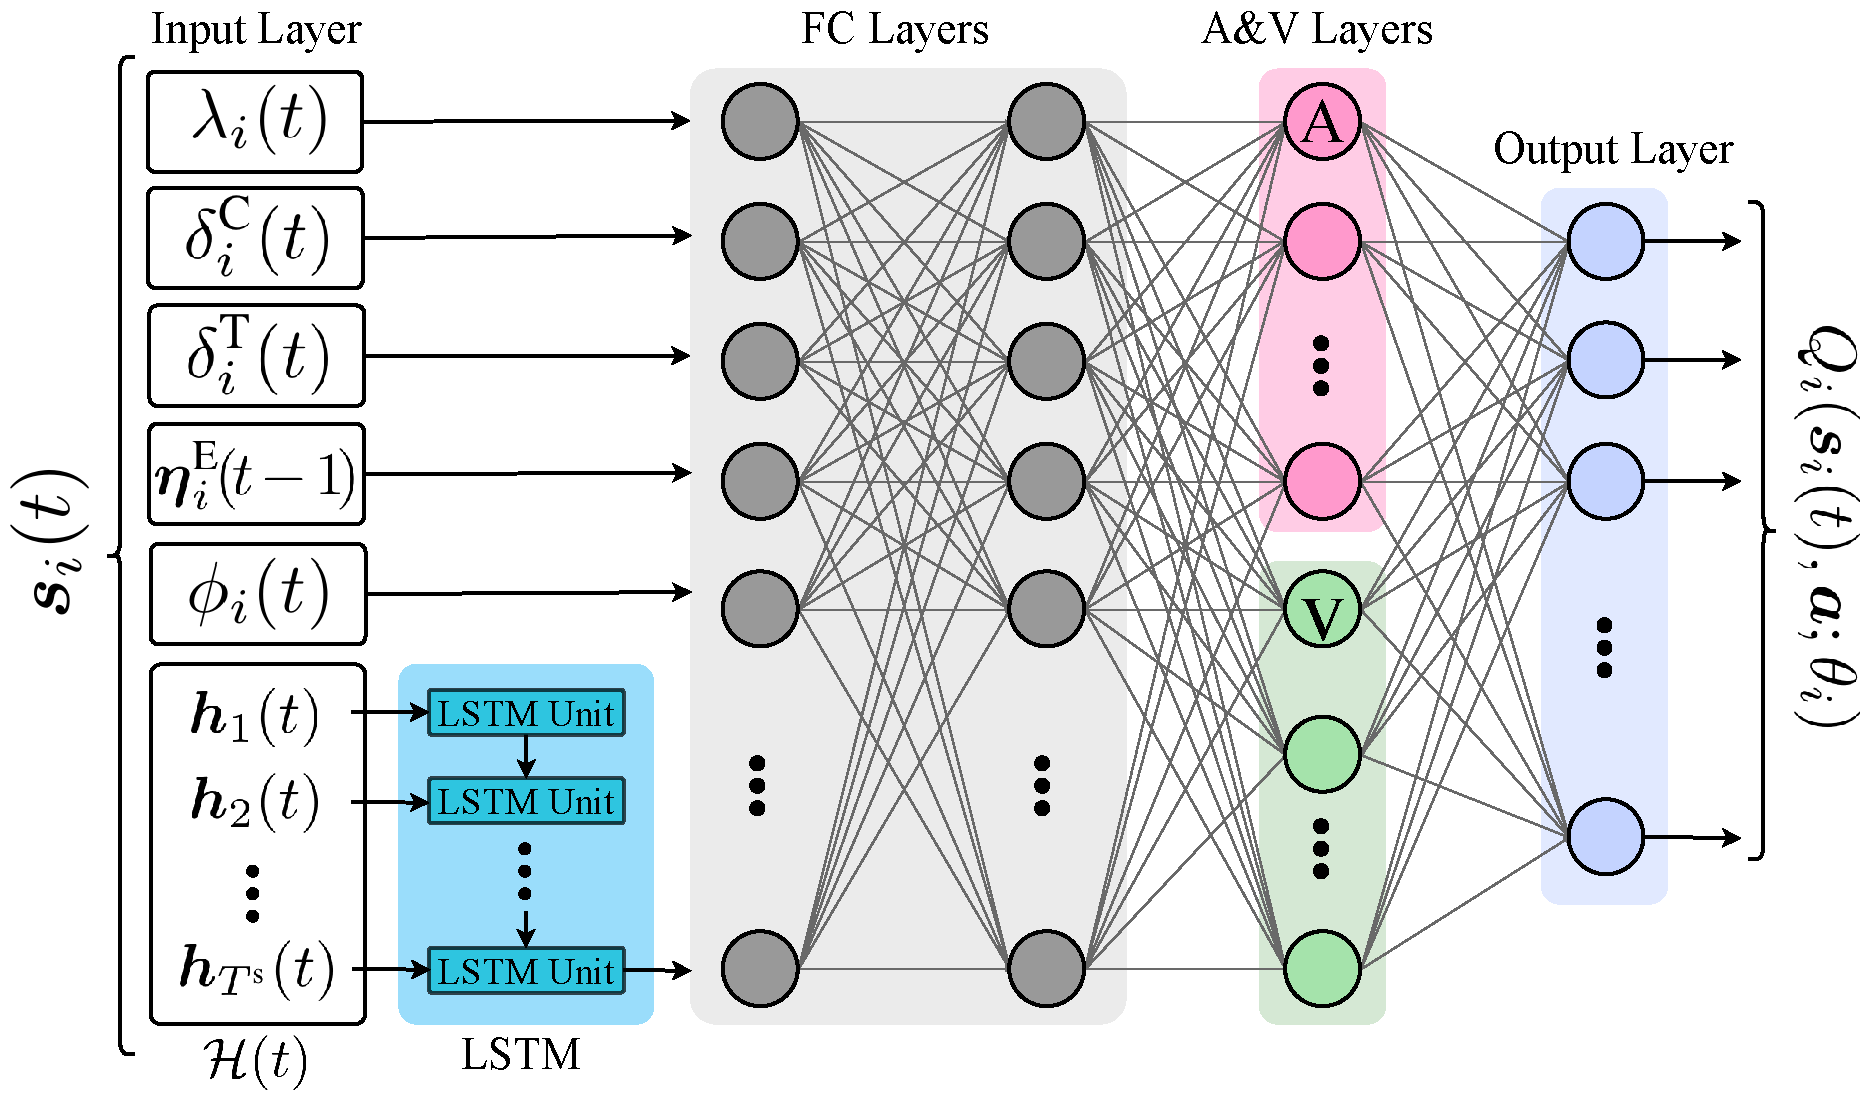
\includegraphics[width=0.7\linewidth]{ DQN}
	\captionsetup{name=Fig.}
	
	\caption{The neural network of MD $i \in \mathcal{I}$, which characterize the Q-value of each action $\boldsymbol{a} \in \mathcal{A}$ under state $\boldsymbol{s}_i(t) \in \mathcal{S}$.}
	\vspace*{-4.5mm}
	\label{DQN}
\end{figure}


\subsection{DQN-based Approach}
We utilize the DQN technique to find the mapping between each state-action pair to Q-values in the formulated MDP. As shown in Fig.~\ref{DQN}, each MD $i \in \mathcal{I}$ is equipped with a neural network comprising six layers. These layers include an input layer, an LSTM layer, two dense layers, an advantage-value (A\&V) layer, and an output layer. The parameter vector $\theta_i$ of MD $i$'s neural network is defined to maintain the connection weights and neuron biases across all layers. For MD $i \in \mathcal{I}$, we utilize the state information as the input of neural network. The state information $\lambda_i(t)$, $\delta_i^{\text{C}}(t)$, $\delta_i^{\text{T}}(t)$, $\phi_i(t)$, and $\boldsymbol{\eta}_i^{\text{E}}(t-1)$ are directly passed to the dense layer, while the state information $\mathcal{H}(t)$ is first supplied to the LSTM layer and then the resulting output is sent to the dense layer. The role and responsibilities of each layer are detailed as follows.


\subsubsection{Predicting Workloads at ENs}
In order to capture the dynamic behavior of workloads at the ENs, we employ the LSTM network \cite{hochreiter1997long}. This network maintains a memory state $\mathcal{H}(t)$ that evolves over time, enabling the neural network to predict future workloads at the ENs based on historical data. By taking the matrix $\mathcal{H}(t)$ as an input, the LSTM network learns the patterns of workload dynamics. The architecture of the LSTM consists of $T^{\text{s}}$ units, each equipped with a set of hidden neurons, and it processes individual rows of the matrix $\mathcal{H}(t)$ sequentially. Through this interconnected design, MD tracks the variations in sequences from $\boldsymbol{h}_1(t)$ to $\boldsymbol{h}_{T^{\text{s}}}(t)$, where vector $\boldsymbol{h}_i(t) = (h_{i,j}(t))_{j \in \mathcal{J}}$, thereby revealing workload fluctuations at the ENs across different time slots. The final LSTM unit produces an output that encapsulates the anticipated workload dynamics, and is then connected to the subsequent layer neurons for further learning.




%\subsubsection{workload Prediction}
%To learning the dynamics of the workloads at the ENs, we use the LSTM network [26], [27], which can keep track of the state $\mathcal{H}(t)$ over time. It can provide the neural network the ability of estimating the workloads at the ENs in the future using the history. The LSTM network takes the matrix $\mathcal{H}(t)$ as input so as to learn the workload dynamics. coresponding the matrix $\mathcal{H}(t)$,  The LSTM network contains $T^{\text{s}}$ LSTM units, each of which contains a set of hidden neurons and takes one row of the matrix $\mathcal{H}(t)$ as input. These LSTM units are connected in sequence so as to keep track of the variations of the sequences from $\{\mathcal{H}(t)\}_1$ to $\{\mathcal{H}(t)\}_{T^{\text{s}}}$, which can reveal the variations of the workloads at the ENs among time slots. The LSTM network will output the information that indicates the dynamics of the workloads in the future in the last LSTM unit, where the output will be connected to the neurons in the next layer for further learning.
%
%---------------------

%This layer is responsible for learning the dynamics of the workloads at the ENs. This is achieved by including an LSTM network [26], [27]. We use the LSTM network because it can keep track of the state $\textbf{H}(t)$ over time. It can provide the neural network the ability of estimating the workloads at the ENs in the future using the history. 
%
%Specifically, the LSTM network takes the matrix $\textbf{H}(t)$ as input so as to learn the workload dynamics. Fig. 3 shows the structure of an LSTM network. The LSTM network contains Tstep LSTM units, each of which contains a set of hidden neurons. Each LSTM unit takes one row of the matrix $\textbf{H}(t)$ as input, we let $\{\textbf{H}(t)\}_1$  denote the $i^{th}$ row of matrix $\textbf{H}(t)$ in Fig. 3. These LSTM units are connected in sequence so as to keep track of the variations of the sequences from $\{\textbf{H}(t)\}_1$ to $\{\textbf{H}(t)\}_{T^{step}}$, which can reveal the variations of the workloads at the ENs among time slots. The LSTM network will output the information that indicates the dynamics of the workloads in the future in the last LSTM unit, where the output will be connected to the neurons in the next layer for further learning.



\subsubsection{State-Action Q-Value Mapping}
The pair of dual dense layers plays a crucial role in learning the mapping of Q-values from the current state and the learned load dynamics to the corresponding actions. The dense layers consist of a cluster of neurons that employ rectified linear units (ReLUs) as their activation functions. In the initial dense layer, connections are established from the neurons in the input layer and the LSTM layer to each neuron in the dense layer. The resulting output of a neuron in the dense layer is connected to each neuron in the subsequent dense layer. In the second layer, the outputs from each neuron establish connections with all neurons in the A\&V layers.



\subsubsection{Dueling-DQN Approach for Q-Value Estimation}
In the neural network architecture, the A\&V layer and the output layer incorporate the principles of the dueling-DQN \cite{wang2016dueling} to compute action Q-values. The fundamental concept of dueling-DQN involves two separate learning components: one for action-advantage values and another for state-value. This approach enhances Q-value estimation by separately evaluating the long-term QoE attributed to states and actions.



The A\&V layer consists of two distinct dense networks referred to as network A and network V. Network A's role is to learn the action-advantage value for each action, while network V focuses on learning the state-value. For an MD $i \in \mathcal{I}$, we define $V_i(\boldsymbol{s}_i(t); \theta_i)$ and $A_i(\boldsymbol{s}_i(t), \boldsymbol{a}; \theta_i)$ to denote the state-value and the action-advantage value of action $\boldsymbol{a} \in \mathcal{A}$ under state $\boldsymbol{s}_i(t) \in \mathcal{S}$, respectively. The parameter $\theta_i$ is responsible for determining these values, and it can be adjusted when training the QECO algorithm.

For an MD $i \in \mathcal{I}$, the A\&V layer and the output layer collectively determine $Q_i(\boldsymbol{s}_i(t), \boldsymbol{a}; \theta_i)$, representing the resulting Q-value under action $\boldsymbol{a} \in \mathcal{A}$ and state $\boldsymbol{s}_i(t) \in \mathcal{S}$, as follows: \vspace{1.7mm}


$Q_i(\boldsymbol{s}_i(t), \boldsymbol{a}; \theta_i) = V_i(\boldsymbol{s}_i(t);\theta_i) +$
\begin{alignat}{1}
	\hspace{0.94cm} \Bigg( A_i(\boldsymbol{s}_i(t),\boldsymbol{a};\theta_i) - {1 \over |\mathcal{A}|} \sum\limits_{\boldsymbol{a}' \in \mathcal{A}}(A_i(\boldsymbol{s}_i(t),\boldsymbol{a}';\theta_i) \Bigg),
	\label{25}  
\end{alignat}
where $\theta_i$ establishes a functional relationship that maps Q-values to pairs of state-action.

%, which characterizes the long-term QoE under any observed state $\boldsymbol{s}_i(t) \in \mathcal{S}$ and action $\mathcal{A} \in \mathcal{A}$. 


%\begin{algorithm} [tbp]
%	\caption{QECO Algorithm (Offloading Decision)}\label{alg:cap}
%	\begin{algorithmic}[1]
	%		\renewcommand{\algorithmicrequire}{\textbf{Input:}} 
	%		\renewcommand{\algorithmicensure}{\textbf{Output:}}
	%		\Require state space $\mathcal{S}$, action space $\mathcal{A}$
	%		\Ensure MD $i \in \mathcal{I}$ experience 
	%		\For {episode 1 to $N^{\text{ep}}$}
	%		\State Initialize $\boldsymbol{s}_i(1)$
	%		\For {time slot $t \in \mathcal{T}$}
	%		\If{MD $i$ receives a new task $z_i(t)$}
	%		\State Send an \textit{UpdateRequest} to EN $j_i$;
	%		\State Receive network parameter vector $\theta_i^{\text{E}}$;
	%		\State Select action $\boldsymbol{a}_i(t)$ based on \eqref{26};
	%		\EndIf
	%		\State Observe a set of QoEs $\{\boldsymbol{q}_i(t'), t' \in \mathcal{F}_i^t\}$;
	%		\State Observe\textcolor{white}{i}the next\textcolor{white}{i}state $\textbf{\textit{s}}_i(t+1)$;\textcolor{white}{i}
	%		\For {each task $z_i(t')$ where $t' \in \mathcal{F}_i^t$} 
	%		\State Send \hspace{-1mm} $(\boldsymbol{s}_i(t'), \boldsymbol{a}_i(t'), \boldsymbol{q}_i(t'), \boldsymbol{s}_i(t'\hspace{-1mm}+1))$ to EN $j_i$;
	%		\EndFor
	%		\EndFor
	%		\EndFor
	%	\end{algorithmic}
%\end{algorithm}


\subsection{QoE-Oriented DRL-Based Algorithm}
\label{section:1}

%Our proposed QoE-Driven DRL-Based Algorithm is designed to efficiently distribute computational loads for training neural networks on MDs while leveraging the support of ENs. The primary objective of this algorithm is to utilize the experience of each MD to train its neural network, allowing the MD to make informed decisions that maximize its long-term QoE. To achieve efficient training, each MD $i \in \mathcal{I}$ is paired with a dedicated EN $n_i \in \mathcal{J}$ that assists in the training process. The selection of EN $n_i$ is based on its maximum transmission capacity with MD $i$. We define the set $\mathcal{I}_j \subset \mathcal{I}$ as the group of MDs whose training is facilitated by EN $j \in \mathcal{J}$.

The QECO algorithm is meticulously designed to optimize the allocation of computational tasks between MDs and ENs. Since the training of neural networks imposes an extensive computational workload on MDs, we enable MDs to utilize ENs for training their neural networks, effectively reducing their computational workload. For each MD $i \in \mathcal{I}$, there is an associated EN, denoted as EN $j_i \in \mathcal{J}$, which assists in the training process. This EN possesses the highest transmission capacity among all ENs. We define $\mathcal{I}_j \subset \mathcal{I}$ as the set of MDs for which training is executed by EN $j \in \mathcal{J}$, i.e. $\mathcal{I}_j = \{i \in \mathcal{I} | j_i = j\}$. This approach is feasible due to the minimal information exchange and processing requirements for training compared to MD's tasks. The algorithms to be executed at MD $i \in \mathcal{I}$ and EN $j \in \mathcal{J}$ are given in Algorithms ~\ref{alg:cap} and ~\ref{alg:cap2}, respectively. The core concept involves training neural networks with MD experiences (i.e., state, action, QoE, next state) to map Q-values to each state-action pair. This mapping allows MD to identify the action in the observed state with the highest Q-value and maximize its long-term QoE.




In detail, EN $j \in \mathcal{J}$ maintains a replay buffer denotes as $\mathcal{M}_i$ with two neural networks for MD $i$: $\textit{Net}_i^{\text{E}}$, denoting the evaluation network, and $\textit{Net}_i^{\text{T}}$, denoting the target network, which have the same neural network architecture. However, they possess distinct parameter vectors $\theta^{\text{E}}_i$ and $\theta^{\text{T}}_i$, respectively. Their Q-values are represented by $Q_i^{\text{E}}(\boldsymbol{s}_i(t), \boldsymbol{a}; \theta^{\text{E}}_i)$ and $Q_i^{\text{T}}(\boldsymbol{s}_i(t), \boldsymbol{a}; \theta^{\text{T}}_i)$ for MD $i \in \mathcal{I}_j$, respectively, associating the action $\boldsymbol{a} \in \mathcal{A}$ under the state $\boldsymbol{s}_i(t) \in \mathcal{S}$. The replay buffer records the observed experience $(\boldsymbol{s}_i(t), \boldsymbol{a}_i(t), \boldsymbol{q}_i(t), \boldsymbol{s}_i(t+1))$ of MD $i$. Moreover, $\textit{Net}_i^{\text{E}}$ is responsible for action selection, while $\textit{Net}_i^{\text{T}}$ characterizes the target Q-values, which represent the estimated long-term QoE resulting from an action in the observed state. The target Q-value serves as the reference for updating the network parameter vector $\theta^{\text{E}}_i$. This update occurs through the minimization of disparities between the Q-values under $\textit{Net}_i^{\text{E}}$ and $\textit{Net}_i^{\text{T}}$. In the following, we introduce the offloading decision algorithm of MD $i \in \mathcal{I}$ and the training process algorithm running in EN $j \in \mathcal{J}$.

% i.e., $\textbf{\textit{s}}_i(1) = \big(\lambda_i(1), \delta_i^{\text{C}}(1), \delta_i^{\text{T}}(1), \boldsymbol{\eta}_i^{\text{E}}(0),\phi_i(1), \mathcal{H}(1) \big)$, where we set $\boldsymbol{\eta}_i^{\text{E}}(0)=0$ for all $j \in \mathcal{J}$, and $ \mathcal{H}(1)$ is a zero matrix with size $T^s \times N$. 




\subsubsection{Offloading Decision Algorithm at MD $i \in \mathcal{I}$}
We analyze a series of episodes, where $N^{\text{ep}}$ denotes the number of them. At the beginning of each episode, if MD $i \in \mathcal{I}$ receives a new task $z_i(t)$, it initializes the state $\mathcal{S}_i(1)$ and sends an $\textit{UpdateRequest}$ to EN $j_i$. After receiving the requested vector $\theta_i^{\text{E}}$ of $\textit{Net}_i^{\text{E}}$ from EN $j_i$, MD $i$ chooses the following action for task $z_i(t)$.
\begin{alignat}{1}
	\hspace*{-2mm}\boldsymbol{a}_i(t) \hspace*{-0.5mm} = \hspace*{-0.5mm}
	\begin{cases} 
		\text{arg $\max_{\boldsymbol{a}\in \mathcal{A}}Q_i^{\text{E}}(\boldsymbol{s}_i(t), \boldsymbol{a}; \theta^{\text{E}}_i)$,} & \text{w.p. $1-\boldsymbol{\epsilon}$,} \\
		\text{pick a random action from $\mathcal{A}$,} & \text{w.p. $\boldsymbol{\epsilon}$,}
	\end{cases}
	\label{26}  
\end{alignat}
where w.p. stands for with probability, and $\boldsymbol{\epsilon}$ represents the random exploration probability. The value of $Q_i^{\text{E}}(\boldsymbol{s}_i(t), \boldsymbol{a}; \theta^{\text{E}}_i)$ indicates the Q-value under the parameter $\theta^{\text{E}}_i$ of the neural network $\textit{Net}_i^{\text{E}}$. Specifically, the MD with a probability of $1 - \boldsymbol{\epsilon}$ selects the action associated with the highest Q-value under $\textit{Net}_i^{\text{E}}$ in the observed state $\boldsymbol{s}_i(t)$.


In the next time slot $t+1$, MD $i$ observes the state $\mathcal{S}_i(t+1)$. However, due to the potential for tasks to extend across multiple time slots, QoE $\boldsymbol{q}_i(t)$ associated with task $z_i(t)$ may not be observable in time slot $t+1$. On the other hand, MD $i$ may observe a group of QoEs associated with some tasks $z_i(t')$ in time slots $t' \leq t$. For each MD $i$, we define the set $\mathcal{F}_i^t \subset \mathcal{T}$ to denote the time slots during which each arriving task $z_i(t')$ is either processed or dropped in time slot $t$, as given by: \vspace{2mm}

$\mathcal{F}_i^t =\bigg \{ t' \bigg|\; t' \leq t,\; \lambda_i(t')>0, \; (1 - x_i(t')) \; l_i^{\text{C}}(t') \; + $ \vspace{-3mm}
\begin{equation}
	\hspace{20mm} x_i(t')\sum\limits_{\mathcal{J}} \sum\limits_{n= t'}^{t}\mathbbm{1}(z_{i,j}^{\text{E}}(n)=z_i(t'))  \; l_{i,j}^{\text{E}}(n) = t \bigg\}.
	\label{27}  
	\nonumber
\end{equation}
Therefore, MD $i$ observes a set of QoEs $\{\boldsymbol{q}_i(t') \mid t' \in \mathcal{F}_i^t\}$ at the beginning of time slot $t+1$, where the set $\mathcal{F}_i^t$ for some $i \in \mathcal{I}$ can be empty. Subsequently, MD $i$ sends its experience $(\boldsymbol{s}_i(t), \boldsymbol{a}_i(t), \boldsymbol{q}_i(t), \boldsymbol{s}_i(t+1))$ to EN $j_i$ for each task $z_i(t')$ in $t' \in \mathcal{F}_i^t$.


%\begin{algorithm}[tbp]
%	\caption{QECO Algorithm (Training Process)}\label{alg:cap2}
%	\begin{algorithmic}[1]
	%		\State Initialize replay buffer $\mathcal{M}_i$ for each MD $i \in \mathcal{I}_j$;
	%		\State Initialize $\textit{Net}_i^{\text{E}}$ and $\textit{Net}_i^{\text{T}}$ with random parameters $\theta_i^{\text{E}}$ and $\theta_i^{\text{T}}$ respectively, for each MD $i \in \mathcal{I}_j$;
	%		\State Set Count := 0
	%		\While{True} \Comment{\textit{infinite loop}}
	%		\If{receive an \textit{UpdateRequest} from MD $i \in \mathcal{I}_j$}
	%		\State Send  $\theta_i^{\text{E}}$ to MD $i \in \mathcal{I}$;
	%		\EndIf
	%		\If {an experience \hspace{-0.2mm} $(\hspace{-0.2mm}\boldsymbol{s}_i(\hspace{-0.2mm}t\hspace{-0.2mm}), \boldsymbol{a}_i(\hspace{-0.2mm}t\hspace{-0.2mm}), \boldsymbol{q}_i(\hspace{-0.2mm}t\hspace{-0.2mm}), \boldsymbol{s}_i(\hspace{-0.2mm}t\hspace{-0.3mm}+\hspace{-0.3mm}\hspace{-0.2mm}1\hspace{-0.2mm}\hspace{-0.2mm})\hspace{-0.2mm})$ is received \\ \;\;\;\; from MD $i \in \mathcal{I}_j$}
	%		\State Store $(\boldsymbol{s}_i(t'), \boldsymbol{a}_i(t'), \boldsymbol{q}_i(t'), \boldsymbol{s}_i(t'\hspace{-1mm}+1))$ in $\mathcal{M}_i$;
	%		\State Get a collection of experiences  $\mathcal{I}$ from $\mathcal{M}_i$; 
	%		\For{each experience $i \in \mathcal{I}$} 
	%		\State Get experience $(\boldsymbol{s}_i(\hspace{-0.2mm}n\hspace{-0.2mm}), \boldsymbol{a}_i(\hspace{-0.2mm}n\hspace{-0.2mm}), \boldsymbol{q}_i(\hspace{-0.2mm}n\hspace{-0.2mm}), \boldsymbol{s}_i(\hspace{-0.2mm}n\hspace{-0.5mm}+1\hspace{-0.2mm}))$; 
	%		\State Generate $\hat{Q}_{i,n}^{\text{T}}$ according to   \eqref{28};
	%		\EndFor
	%		\State Set vector  $\hat{\mathbf{Q}}_i^{\text{T}} := (\hat{Q}^{\text{T}}_{i,n})_{n \in \mathcal{N}}$;
	%		\State Update $\theta_i^{\text{E}}$ to minimize $L(\theta_i^{\text{E}}$, $\hat{\mathbf{Q}}_i^{\text{T}})$ in   \eqref{30};
	%		\State Count := Count + 1;
	%		\If {mod(Count, \textit{ReplaceThreshold}) = 0}
	%		\State $\theta_i^{\text{T}}$ := $\theta_i^{\text{E}}$;
	%		\EndIf
	%		\EndIf
	%		\EndWhile
	%		
	%	\end{algorithmic}
%\end{algorithm}


\subsubsection{Training Process Algorithm at EN $j \in \mathcal{J}$}
Upon initializing the replay buffer $\mathcal{M}_i$ with the neural networks $\textit{Net}_i^{\text{E}}$ and $\textit{Net}_i^{\text{T}}$ for each MD $i \in \mathcal{I}_j$, EN $j \in \mathcal{J}$ waits for messages from the MDs in the set $\mathcal{I}_j$. When EN $j$ receives an $\textit{UpdateRequest}$ signal from an MD $i \in \mathcal{I}_j$, it responds by transmitting the updated parameter vector $\theta^{\text{E}}_i$, obtained from $\textit{Net}_i^{\text{E}}$, back to MD $i$. On the other side, if EN $j$ receives an experience $(\boldsymbol{s}_i(t), \boldsymbol{a}_i(t), \boldsymbol{q}_i(t), \boldsymbol{s}_i(t+1))$ from MD $i \in \mathcal{I}_j$, the EN stores this experience in the replay buffer $\mathcal{M}_i$ associated with that MD. %The replay buffer operates at maximum capacity and FIFO principle.

The EN randomly selects a sample collection of experiences from the replay buffer, denoted as $\mathcal{N}$. For each experience $n \in \mathcal{N}$, it calculates the value of $	\hat{Q}^{\text{T}}_{i,n}$. This value represents the QoE in experience $n$ and includes a discounted Q-value of the action anticipated to be taken in the subsequent state of experience $n$, according to the network $\textit{Net}^\text{T}_i$, given by
\begin{alignat}{1}
	\hat{Q}_{i,n}^{\text{T}} = \boldsymbol{q}_i(n) + \gamma Q_i^{\text{T}}(\boldsymbol{s}_i(n+1)), \tilde{\boldsymbol{a}}_n; \theta_i^{\text{T}}),
	\label{28}  
\end{alignat}  
where $\tilde{\boldsymbol{a}}_n$ denotes the optimal action for the state $\boldsymbol{s}_i(n+1)$ based on its highest Q-value under $\textit{Net}_i^{\text{E}}$, as given by:
\begin{alignat}{1}
	\tilde{\boldsymbol{a}}_n = \text{arg} \; \max_{\boldsymbol{a} \in \mathcal{A}} \; Q_i^{\text{E}}(\boldsymbol{s}_i(n+1), \boldsymbol{a}; \theta_i^{\text{E}}).
	\label{29}  
\end{alignat} 
In particular, regarding experience $n$, the target-Q value $\hat{Q}_{i,n}^{\text{T}}$ represents the long-term QoE for action $\boldsymbol{a}_i(n)$ under state $\boldsymbol{s}_i(n)$. This value corresponds to the QoE observed in experience $n$, as well as the approximate expected upcoming QoE. %based on $\textit{Net}_i^{\text{T}}_i$, i.e., $\gamma Q_i^{\text{T}}(\mathcal{S}_i(i+1)), \mathcal{A}_i^{\text{N}}; \theta_i^{\text{T}})$
Based on the set $\mathcal{N}$, the EN trains the MD's neural network using previous sample experiences. Simultaneously, it updates $\theta^{\text{E}}_i$ in $\textit{Net}_i^{\text{E}}$ and computes vector $\hat{\mathbf{Q}}_i^{\text{T}} = (\hat{Q}^{\text{T}}_{i,n})_{n \in \mathcal{N}}$. The key idea of updating $\textit{Net}_i^{\text{E}}$ is to minimize the disparity in Q-values between $\textit{Net}_i^{\text{E}}$ and $\textit{Net}_i^{\text{T}}$, as indicated by the following loss function:
\begin{alignat}{1}
	\hspace{-2mm}L(\theta_i^{\text{E}},\hat{\mathbf{Q}}_i^{\text{T}}) = {1 \over |\mathcal{N}| }\hspace{-1mm} \sum\limits_{n \in \mathcal{N}} \bigg(Q_i^{\text{E}}(\boldsymbol{s}_i(n) , \boldsymbol{a}_i(n); \theta_i^{\text{E}} ) -   \hat{Q}^{\text{T}}_{i,n}  \bigg)^2.
	\label{30}  
\end{alignat}  
In every \textit{ReplaceThreshold} iterations, the update of $\textit{Net}_i^{\text{T}}$ will involve duplicating the parameters from $\textit{Net}_i^{\text{E}}$ ($\theta_i^{T} = \theta_i^{E}$). The objective is to consistently update the network parameter $\theta_i^{T}$ in $\textit{Net}_i^{\text{T}}$, which enhances the approximation of the long-term QoE when computing the target Q-values in \eqref{28}.\\

\subsubsection{Computational Complexity}


The computational complexity of the QECO algorithm is determined by the number of experiences required to discover the optimal offloading policy. Each experience involves backpropagation for training, which has a computational complexity of $\mathcal{O}(C)$, where $C$ represents the number of multiplication operations in the neural network. During each training round triggered by the arrival of a new task, a sample collection of experiences of size $|\mathcal{N}|$ is utilized from the replay buffer. Since the training process encompasses $N^{\text{ep}}$ episodes and there are $K$ expected tasks in each episode, the computational complexity of the proposed algorithm is $\mathcal{O}(N^{\text{ep}}K|\mathcal{N}|C$), which is polynomial. Given the integration of neural networks for function approximation, the convergence guarantee of the DRL algorithm remains an open problem. In this work, we will empirically evaluate the convergence of the proposed algorithm in Section \ref{section:2}.

%Regarding the convergence, as mentioned in many existing works (e.g., [29]), the convergence guarantee of a DRL algorithm is still an open problem. Despite the fact that the convergence of a reinforcement learning algorithm can be proven, a DRL algorithm requires function approximation (e.g., the approximation of the Q-values in deep Q-learning algorithm) using neural networks, under which the convergence may no longer be guaranteed. In this work, we empirically evaluate the convergence performance of the proposed algorithm in Section 5.1.



\section{Performance Evaluation}\label{section:V}
In this section, we first present the simulation setup and training configuration. We then illustrate the convergence of the proposed DRL-based QECO algorithm and evaluate its performance in comparison to three baseline schemes in addition to the existing work~\cite{yang2018distributed}.
%We begin by presenting the simulation setting and training configuration, followed by the evaluation of QECO algorithm under multiple key performance metrics in comparison to benchmark methods.


\subsection{Simulation Setup}
We consider a MEC environment with 50 MDs and 5 ENs, similar to \cite{9253665}. We also follow the model presented in \cite{zhou2021deep} to determine the energy consumption. All the parameters are given in Table~\ref{table}. To train the MDs' neural networks, we adopt a scenario comprising 1000 episodes. Each episode contains 100 time slots, each of length 0.1 second. The QECO algorithm incorporates real-time experience into its training process to continuously enhance the offloading strategy. Specifically, we employ a batch size of 16, maintain a fixed learning rate of 0.001, and set the discount factor $\gamma$ to 0.9. The probability of random exploration gradually decreases from an initial value 1, progressively approaching 0.01, all of which is facilitated by an RMSProp optimizer. %The convergence of the proposed algorithm is evaluated across a spectrum of neural network hyperparameters and algorithm configurations.




%In these simulations, we first evaluate the QECO algorithm for each of the influencing QoE factors, including the number of completed tasks, overall energy consumption, and average delay. Subsequently, we demonstrate the overall improvement of QECO in terms of average QoE by comparing it against the following benchmark methods across multiple challenging scenarios.
We use the following methods as benchmarks.
\begin{enumerate}
	
	\item \textbf{Local Computing (LC):} The MDs execute all of their computation tasks using their own computing capacity.
	
	\item \textbf{Full Offloading (FO):} Each MD dispatches all of its computation tasks while choosing the offloading target randomly. %It leverages their complete communication capacity and the computation resources allocated to them by the EN.
	
	\item \textbf{Random Decision (RD):} In this approach, when an MD receives a new task, it randomly makes the offloading decisions and selects the offloading target if it decides to dispatch the task. %This method leverages the MD's complete computational and communication capabilities, and the computational resources allocated to it by the EN.
	
	\item \textbf{PGOA~\cite{yang2018distributed}:} This existing method is a distributed optimization algorithm designed for delay-sensitive tasks in an environment where MDs interact strategically with multiple ENs. We select PGOA as a benchmark method due to its similarity to our work.
\end{enumerate}

%In this part, we first illustrate the convergence performance of the proposed DRL-based QECO algorithm, and then we compare its performance of these two proposed methods with the fiducial methods in terms of the energy con- sumption of the system and the average delay of the task at each time slot.

%In the following, we first show the convergence of the proposed algorithm across episodes. Then, we compare the performance of our proposed algorithm with the benchmark methods under different parameter settings.

%In the following, we will compare the performance of the QECO algorithm with benchmark methods under two different computation workloads. This comparison will involve increasing the task arrival rate and the number of MDs.



%\newpage

%\begin{table}
%	\centering
%	\renewcommand{\arraystretch}{1}
%	\captionsetup{name=TABLE}
%	\caption{Simulation Parameters}
%	\scalebox{1}{%
%		\begin{tabular}{ l|l } 
%			%\toprule
%			\textbf{Parameter} & \textbf{Value}  \\ \hline
%			%\midrule
%			%Number of MDs $i$  & 50  \\ 
%			%Number of EN $j$  & 5  \\ 
%			%Number of episodes $N^{\text{ep}}$  & 1000  \\ 
%			%Number of time slots $T$  & 100 (with $\tau = 0.1$ second) \\ 
%			Computation capacity of MD $f_i$  & 2.6 GHz \\ 
%			Computation capacity of EN $f_j^{\text{E}}$ & 42.8 GHz  \\ 
%			Transmission capacity of MD $r_{i,j}(t)$ & 14 Mbps  \\ 
%			Task arrival rate & 150 Task/sec  \\ 
%			Size of task $\lambda_i(t)$  & $\{\text{1.0, 1.1, \ldots , 7.0}\}$ Mbits \\ 
%			Required CPU cycles of task $\rho_i(t)$  & $\{\text{0.197,0.297,0.397}\}$ $\times10^3$ \\ 
%			Deadline of task $ \Delta_i$  & 10 time slots (1 Sec)\\ 
%			Battery level percentage of MD $\phi_i(t)$  & $\{\text{25, 50, 75}\}$\\ %Percent \\ 
%			%Computation power of MD $p_i^{\text{C}}$ & \text{$10^{-27}(f_i)^3$}  \\ 
%			Computation power of EN $p_j^{\text{E}}$ & 5 W  \\ 
%			Transmission power of MD $p_i^{\text{T}}$ & 2.3 W  \\ 
%			Standby power of MD $p_i^{\text{I}}$& 0.1 W  \vspace{1mm}\\ 
%			%\toprule
%	\end{tabular}}
%	\label{table}
%\end{table}

\subsection{Performance Comparison and Convergence}
\label{section:2}





%We evaluate the convergence of the proposed algorithm under different neural network hyperparameters and algorithm settings.

%We first investigate the effects of different hyper-parameters on the convergence performance of the proposed QECO algorithm, which is shown through the average QoE across episodes. In Fig. \ref{chart0} (a) the convergence of the proposed algorithm under different values of learning rate is shown, where the learning rate controls the step size in each iteration for moving towards the minimum of the loss function. %It can be observed that the average QoE in each episode increases rapidly as the training episodes increase, and the efficient computation offloading policies can be successfully learned as the interaction continues.
% In Fig. \ref{chart0} (a), learning rate = 0.001 leads to a relatively fast convergence and small converged cost. When the learning rate is small (i.e., 0.0001), the convergence is slow and the converged cost increases and also a too big learning rate cause poor convergence performance. Fig. \ref{chart0} (b) shows the convergence performance under different value of batch sizes, which refers to the number of sampled experiences in each training round. We vary the value of batch size of each MD from 4 to 16, batch size as 16 has the best convergence performance. As it further increases, the performance of the proposed algorithm does not have a significant improvement in terms of the convergence speed and the converged result. We set the default values of batch size for each MD as 16.



%Fig. 4 (b) shows the algorithm performance under differ- ent batch sizes, i.e., the number of experiences sampled in each training round. As the batch size increases from 2 to 8, the convergence speed increases. As it further increases from 8 to 32, the performance of the proposed algorithm does not have a significant improvement in terms of the convergence speed and the converged result. Thus, we can choose a small batch size (e.g., 8) to reduce the time for one round of training without significantly reducing the performance of the proposed algorithm.

%lr = 103 leads to a relatively fast convergence and small converged cost.

%Based on the parameters given in Table \ref{table}, the learning process commences with random policy, and after about 400 episodes, the proposed algorithm achieves an average QoE of 0.77. 

%We first delve into the investigation of the convergence performance of the proposed QECO algorithm, which is shown through the average QoE across episodes in Fig. \ref{chart0} (a). 




%This represents a notable enhancement of 77\% and 16\% over LC and PGOA, respectively. This improvement is attributed to our algorithm's ability to reduce each user-associated cost regarding \eqref{28}, while striving to increase the number of completed tasks. As shown in Figs. \ref{chart0} (b), the converged QECO algorithm decreases the average cost by 38\% compared to RD and 25\% compared to PGOA.


%\subsection{Method Comparison}
%In this part, we first investigate the performance of the proposed DRL-based algorithm under different computation workloads in comparison to benchmark methods across several key performance metrics, including the number of completed tasks, average delay, and energy consumption in the entire system. Then, we evaluate the average QoE of users, which is a balance among these metrics with meticulous attention to users' demands.


We first evaluate the number of completed tasks when comparing our proposed QECO algorithm with the other four schemes. As illustrated in Fig.~\ref{chart1} (a), the QECO algorithm consistently outperforms the benchmark methods when we vary the task arrival rate. At a lower task arrival rate (i.e., 50), most of the methods demonstrate similar proficiency in completing tasks. However, as the task arrival rate increases, the efficiency of QECO becomes more evident. Specifically, when the task arrival rate increases to 250, our algorithm can increase the number of completed tasks by 73\% and 47\% compared to RD and PGOA, respectively.
Similarly, in Fig.~\ref{chart1} (b), as the number of MDs increases, QECO shows significant improvements in the number of completed tasks compared to other methods, especially when faced with a large number of MDs. When there are 110 MDs, our proposed algorithm can effectively increase the number of completed tasks by at least 34\% comparing with other methods. This achievement is attributed to the QECO's ability to effectively handle unknown workloads and prevent congestion at the ENs.

Figs.~\ref{chart2} (a) and ~\ref{chart2} (b) illustrate the overall energy consumption for different values of task arrival rate and the number of MDs, respectively. At the lower task arrival rate, the total energy consumption of all methods is close to each other. The total energy consumption increases when we have a higher task arrival rate.  
%When the task arrival rate increases, the total energy consumption of each method increases differently. It can be found that the production of more computational tasks leads to a continuous increase in energy consumption until the capacity is saturated, and the energy consumption remains constant at its maximum. The QECO algorithm takes into account the battery level of the MD in its decision-making process. 
As can be observed from Fig.~\ref{chart2} (a), at task arrival rate 450, QECO effectively reduces overall energy consumption by 18\% and 15\% compared to RD and PGOA, respectively, as it takes into account the battery level of the MD in its decision-making process. However, it consumes more energy compared to LC and FO because they do not utilize all computing resources. In particular, LC only uses the MD's computational resources, while FO utilizes the allocated EN computing resources.

\begin{figure}[tbp]
	\centering
	\captionsetup{name=Fig.}
	\begin{minipage}[b]{0.34\linewidth}
		\centering
		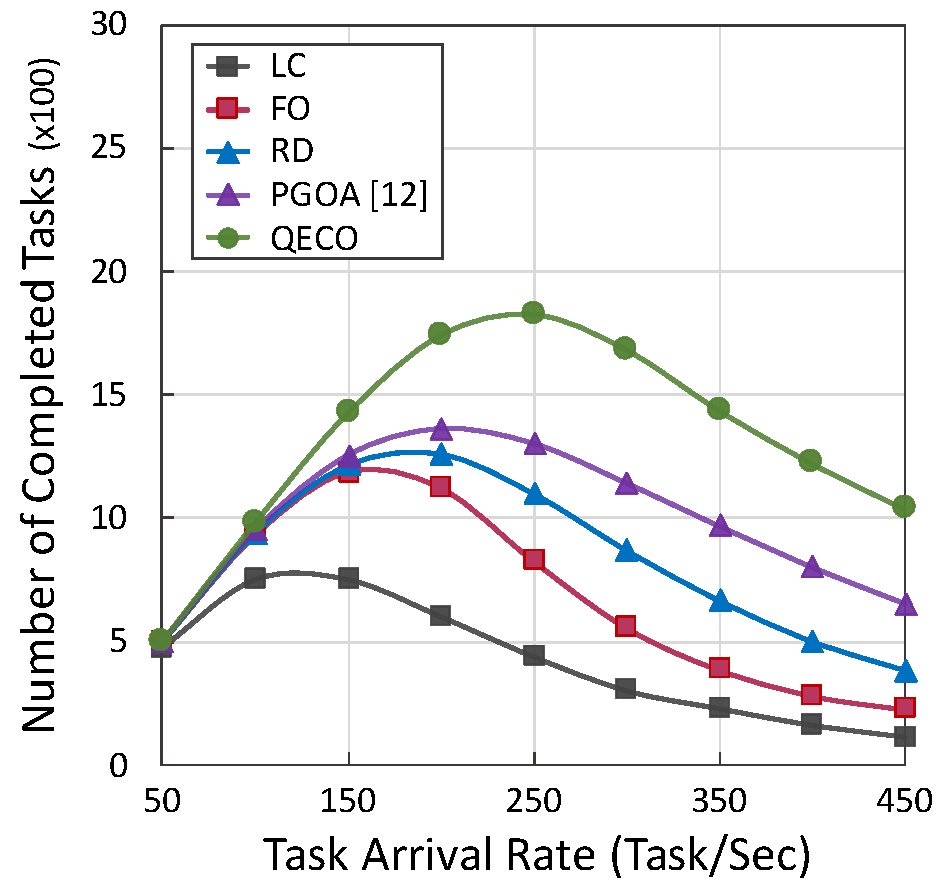
\includegraphics[width=\textwidth]{ completed_tasks_1} 
		\textcolor{white}{i}\hspace{0.6cm}(a)
	\end{minipage}
	\hspace{-0.2cm}
	\begin{minipage}[b]{0.34\linewidth}
		\centering
		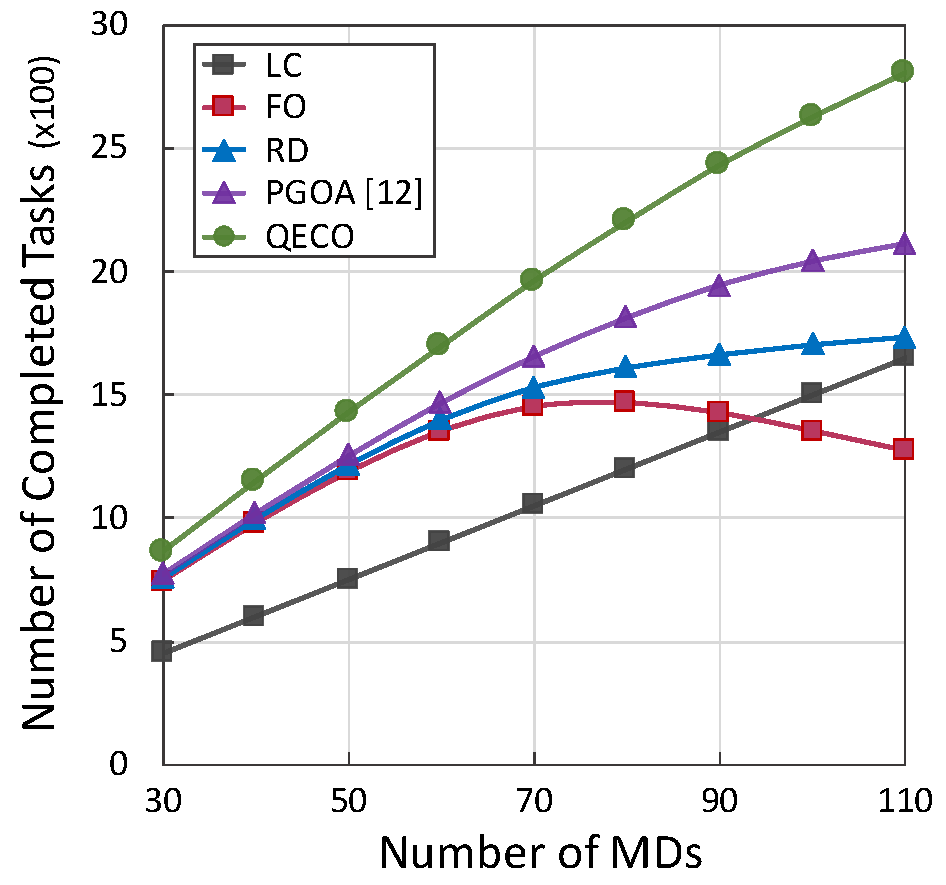
\includegraphics[width=\textwidth]{ completed_tasks_2}
		\textcolor{white}{i}\hspace{0.6cm}(b)
	\end{minipage}
	%\vspace{-0.65cm}
	\caption{The number of completed tasks under different computation workloads: (a) task arrival rate; (b) the number of MDs.}
	\label{chart1}
\end{figure}



\begin{figure}[tbp]
	\centering
	\captionsetup{name=Fig.}
	\begin{minipage}[b]{0.340\linewidth}
		\centering
		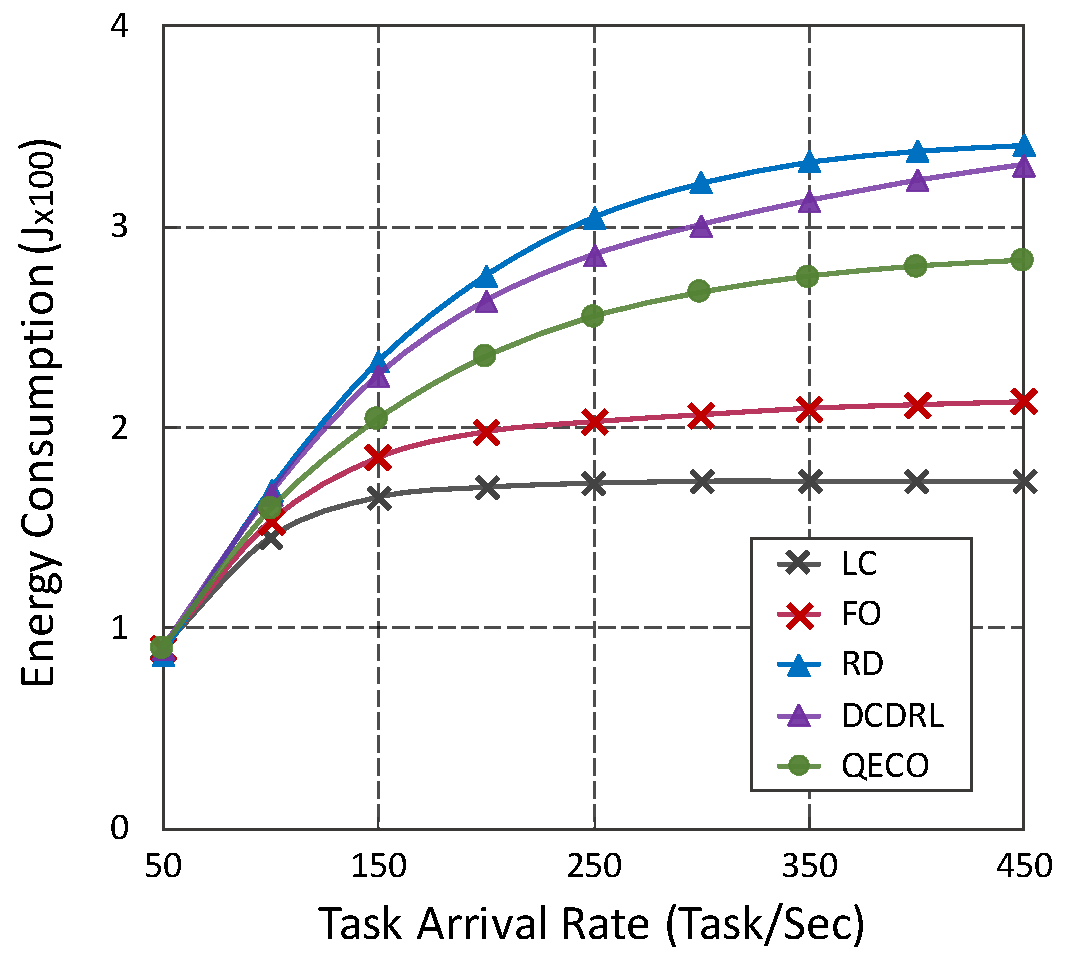
\includegraphics[width=\textwidth]{ energy_1} 		
		\textcolor{white}{i}\hspace{0.6cm}(a)
	\end{minipage}
	%\hspace{-0.2cm}
	\begin{minipage}[b]{0.340\linewidth}
		\centering
		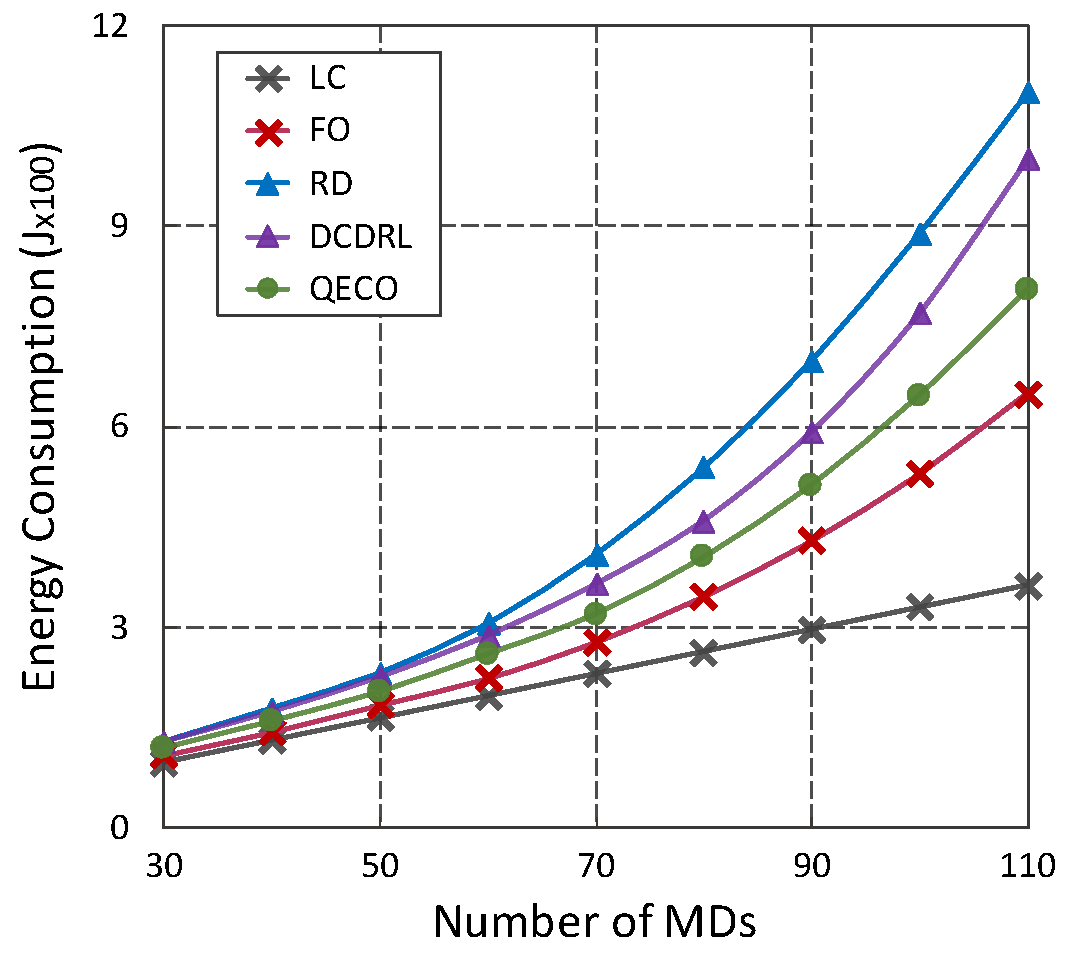
\includegraphics[width=\textwidth]{ energy_2}
		\textcolor{white}{i}\hspace{0.6cm}(b)
	\end{minipage}
	%\vspace{-0.7cm}
	\caption{The overall energy consumption under different computation workloads: (a) task arrival rate; (b) the number of MDs.}
	\label{chart2}
\end{figure}

\begin{figure}[t]
	\centering
	\captionsetup{name=Fig.}
	\begin{minipage}[b]{0.340\linewidth}
		\centering
		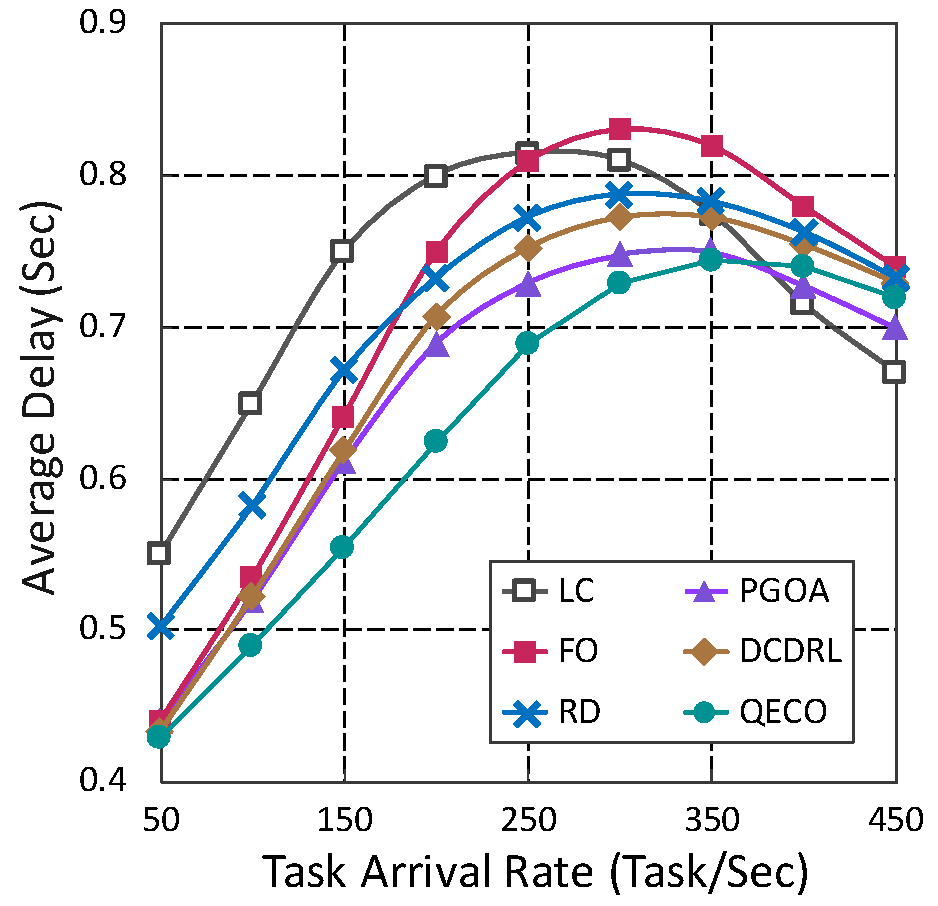
\includegraphics[width=\textwidth]{ delay_1} 		
		\textcolor{white}{i}\hspace{0.6cm}(a)
	\end{minipage}
	\hspace{-0.2cm}
	\begin{minipage}[b]{0.340\linewidth}
		\centering
		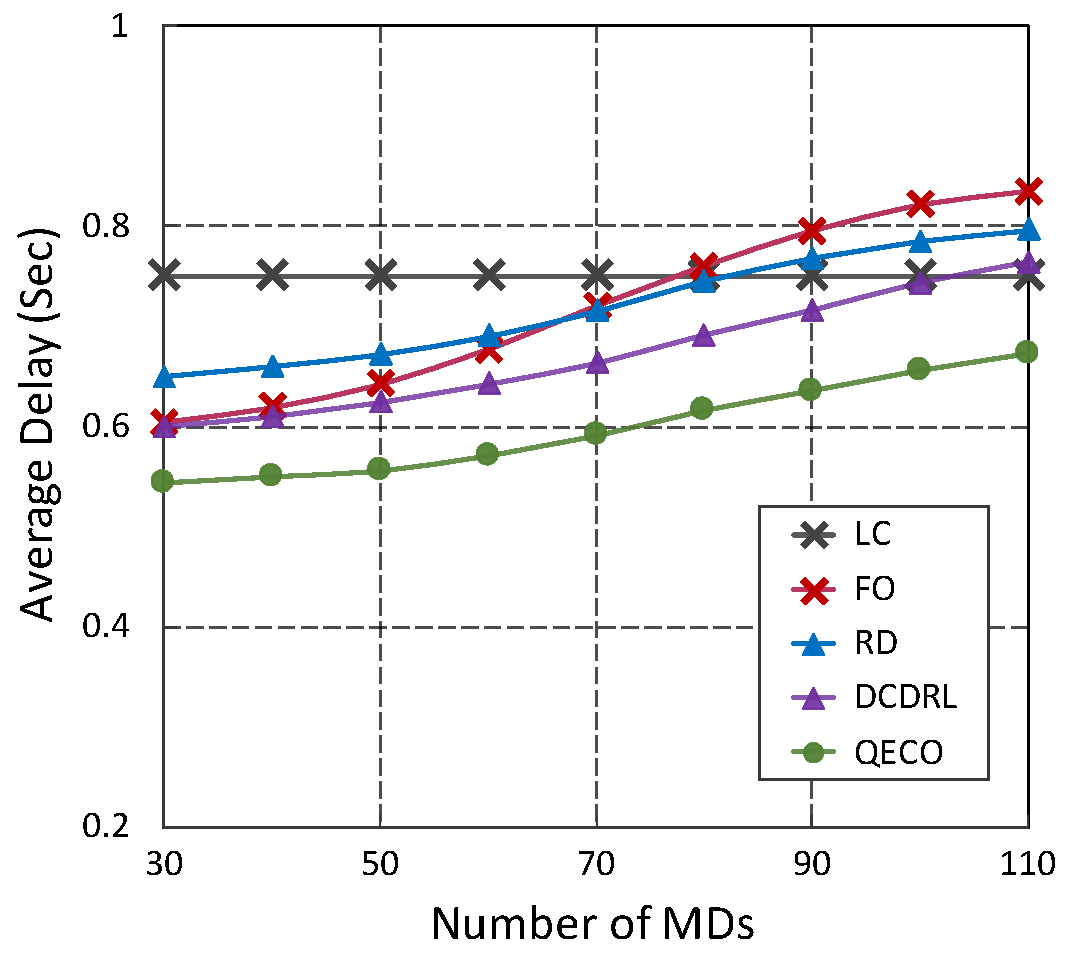
\includegraphics[width=\textwidth]{ delay_2}
		\textcolor{white}{i}\hspace{0.6cm}(b)
	\end{minipage}
	%\vspace{-0.7cm}
	\caption{The average delay under different computation workloads: (a) task arrival rate; (b) the number of MDs.}
	\label{chart3}
\end{figure} 

\begin{figure}[tbp]
	\centering
	\captionsetup{name=Fig.}
	\begin{minipage}[b]{0.340\linewidth}
		\centering
		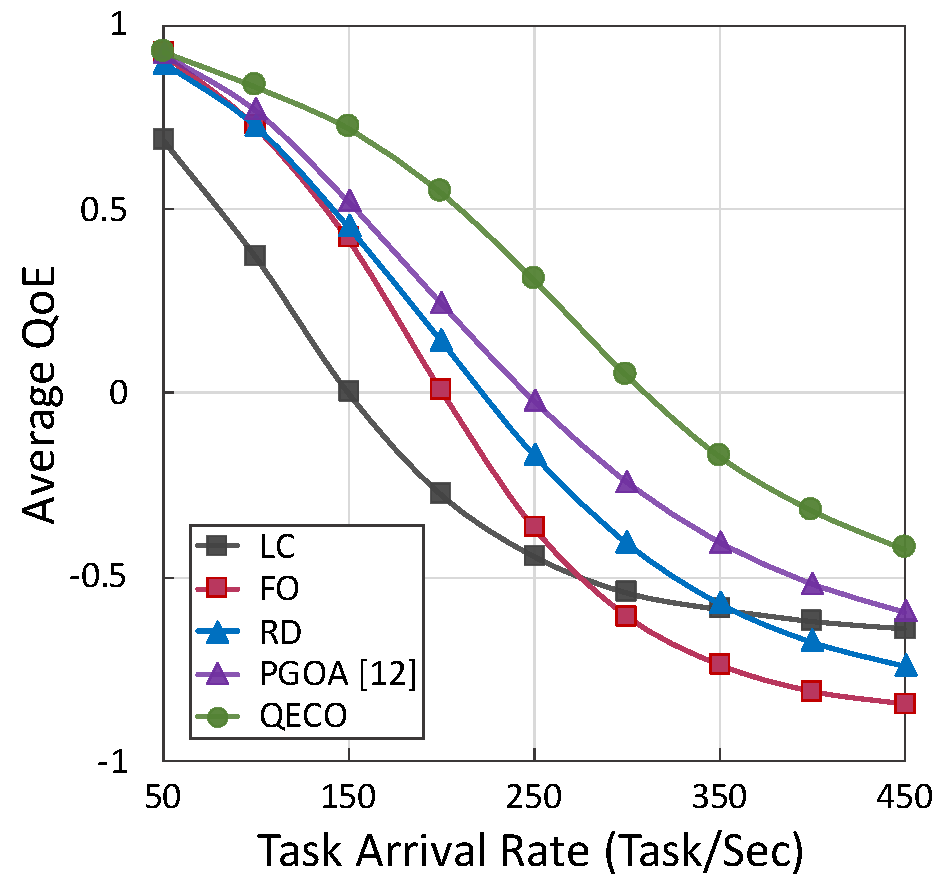
\includegraphics[width=\textwidth]{ qoe_1} 		
		\textcolor{white}{i}\hspace{0.6cm}(a)
	\end{minipage}
	\hspace{-0.2cm}
	\begin{minipage}[b]{0.340\linewidth}
		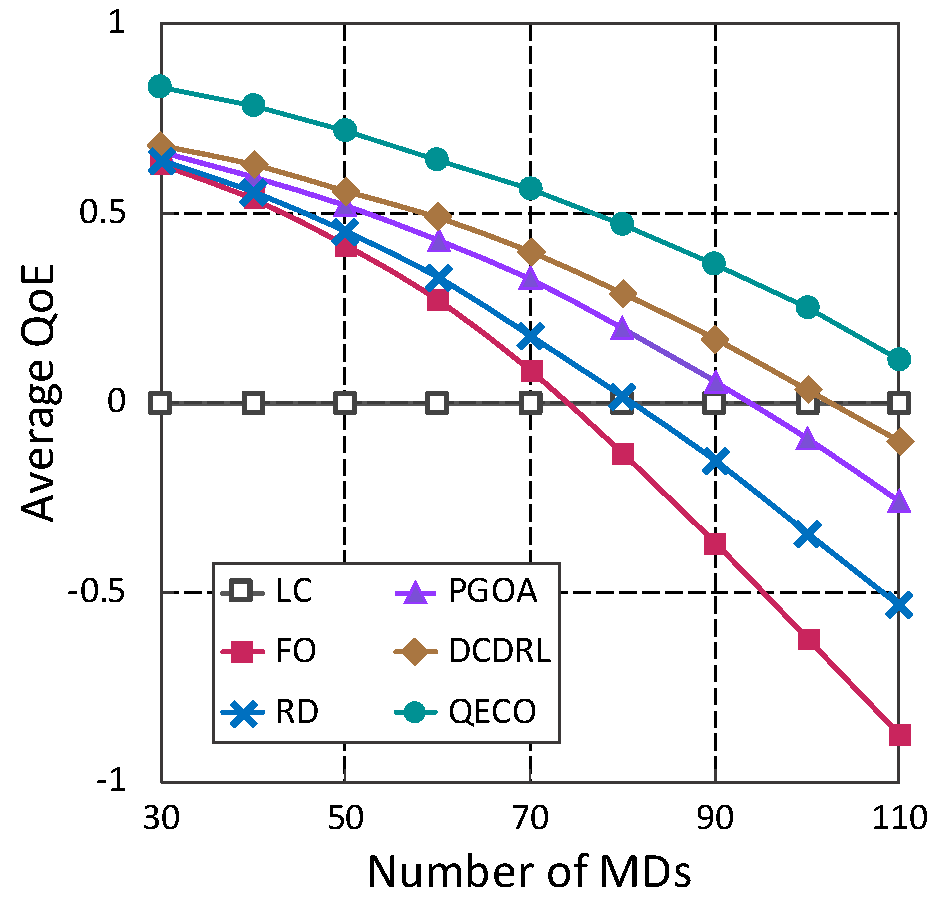
\includegraphics[width=\textwidth]{ qoe_2}
		\textcolor{white}{i}\hspace{0.6cm}(b)
	\end{minipage}
	%\vspace{-0.7cm}
	\caption{The average QoE under different computation workloads: (a) task arrival rate; (b) the number of MDs.}
	\label{chart4}
\end{figure} 





In Fig.~\ref{chart2} (b), an increasing trend in overall energy consumption is observed as the number of MDs increases since the number of resources available in the system increases, which leads to higher energy consumption. The QECO algorithm consistently outperforms RD and PGOA methods in overall energy consumption, especially when there are a large number of MDs. Specifically, QECO demonstrates a 27\% and 16\% reduction in overall energy consumption compared to RD and PGOA, respectively, when the number of MDs increases to 110.

As shown in Fig.~\ref{chart3} (a), the QECO algorithm maintains a lower average delay compared to other methods as the task arrival rate increases from 50 to 350. Specifically, when the task arrival rate is 200, it reduces the average delay by at least 12\% compared to other methods. However, for task arrival rates exceeding 350, QECO may experience a higher average delay compared to some of the other methods. This can be attributed to the fact that the other algorithms drop more tasks while our proposed algorithm is capable of completing a higher number of tasks, potentially leading to an increase in average delay. In Fig.~\ref{chart3} (b), as the number of MDs increases, we observe a rising trend in the average delay. It can be inferred that an increase in computational load in the system can lead to higher queuing delays and computations at ENs. Considering the QECO's ability to schedule workloads, when the number of MDs increases from 30 to 110, it consistently maintains a lower average delay which is at least 8\% less than the other methods.

%Fig. 6 illustrates a performance comparison of methods in terms of energy consumption in the entire system, considering an increase in the task arrival rate and the number of MDs. With efficient decision-making, the DRL-based algorithm achieves lower energy consumption in both cases compared to RD and PGOA. However, it consumes more energy compared to LC and FC. This is because LC only utilizes the MD's computational resources, and FC solely utilizes the transmission link. In Fig. 6(a), when the task arrival rate is low, the energy consumption of all methods is close to each other, and as the task arrival rate increases, the energy consumption of each method also increases. It can be observed that the generation of more computational tasks leads to a continuous increase in energy consumption. When the task arrival rate increases from 0.1 to 0.9, the DRL-based algorithm increases by 20\%, while RD and PGOA increase by at least 30\%. Similarly, in Fig. 6(b), the DRL-based algorithm effectively reduces energy consumption, especially when the number of MDs is large.The DRL-based algorithm demonstrates a 15\% reduction in energy consumption compared to RD and a 30\% reduction compared to PGOA as the number of MDs increases to 110.

%In the following, we delve into the investigation of the overall improvement achieved by the QECO algorithm in comparison to other methods in terms of the average QoE as the task arrival rate and the number of MDs increase. This metric signifies the average advantage created by each method for MDs, including a combination of the values of the previously evaluated metrics (task completion, delay, energy consumption) according to the demands of MDs.

%The average QoE comparison in Fig.~\ref{chart4} (a) indicates the superiority of the QECO algorithm in providing MDs with a better experience. By taking into account the specific demands of MDs for each key performance metric, it consistently achieves a higher average QoE across various values of arrival task rates when compared to other methods. Specifically, when the task arrival rate is moderate (i.e., 250), QECO increases the average QoE by 57\% and 33\% compared to RD and PGOA, respectively. In Fig.~\ref{chart4} (b), As the number of MDs increases, the potential workload on the ENs also rises, leading to a decrease in the average QoE for each method (excluding LC). It can be observed that an increase in the ENs' workload leads to a reduction in the allocated computing capacity for MDs, resulting in a decrease in the average QoE. However, QECO effectively manages the uncertain load at the ENs. When the number of MDs increases to 90, it increases the average QoE by at least 29\% more than the other methods.

We further investigate the overall improvement achieved by the QECO algorithm in comparison to other methods in terms of the average QoE. This metric signifies the advantages MDs obtain by utilizing different algorithms. Fig.~\ref{chart4} (a) shows the average QoE for different values of task arrival rate. This figure indicates the superiority of the QECO algorithm in providing MDs with an enhanced experience. Specifically, when the task arrival rate is moderate (i.e., 250), QECO improves the average QoE by 57\% and 33\% compared to RD and PGOA, respectively. Fig.~\ref{chart4} (b) illustrates the average QoE when we increase the number of MDs. The EN's workload grows when there are a larger number of MDs, leading to a reduction in the average QoE of all methods except LC. However, QECO effectively manages the uncertain load at the ENs. When the number of MDs increases to 90, QECO achieves at least a 29\% higher QoE comparing with the other methods.
It is worth noting that although improvements in each of the QoE factors can contribute to enhancing system performance, it is essential to consider the user's demands in each time slot. Therefore, the key difference between QECO and other methods is that it prioritizes users' demands, enabling it to strike an appropriate balance among them, ultimately leading to a higher QoE for MDs.








We finally delve into the investigation of the convergence performance of the QECO algorithm, which is shown through the average QoE across episodes in Figs.~\ref{chart0} (a) and~\ref{chart0} (b). We explore the impact of two main hyper-parameters on the convergence speed and the converged result of the proposed algorithm. Fig. \ref{chart0} (a) illustrates the convergence of the proposed algorithm under different learning rates, where the learning rate regulates the step size per iteration towards minimizing the loss function. The QECO algorithm achieves an average QoE of 0.77 after around 400 episodes when the learning rate is 0.001, indicating relatively rapid convergence. However, with smaller learning rates (e.g., 0.0001) or larger values (e.g., 0.01),  a slower convergence is observed. Fig. \ref{chart0} (b) shows the convergence of the proposed algorithm under different batch sizes, which refer to the number of sampled experiences in each training round. An improvement in convergence performance is observed as the batch size increases from 4 to 16. However, further increasing the batch size from 16 to 32 does not notably enhance the converged QoE or convergence speed. Hence, a batch size of 16 may be more appropriate for training processes.

\begin{figure}
	\centering
	\captionsetup{name=Fig.}
	\begin{minipage}[b]{0.34\linewidth}
		\centering
		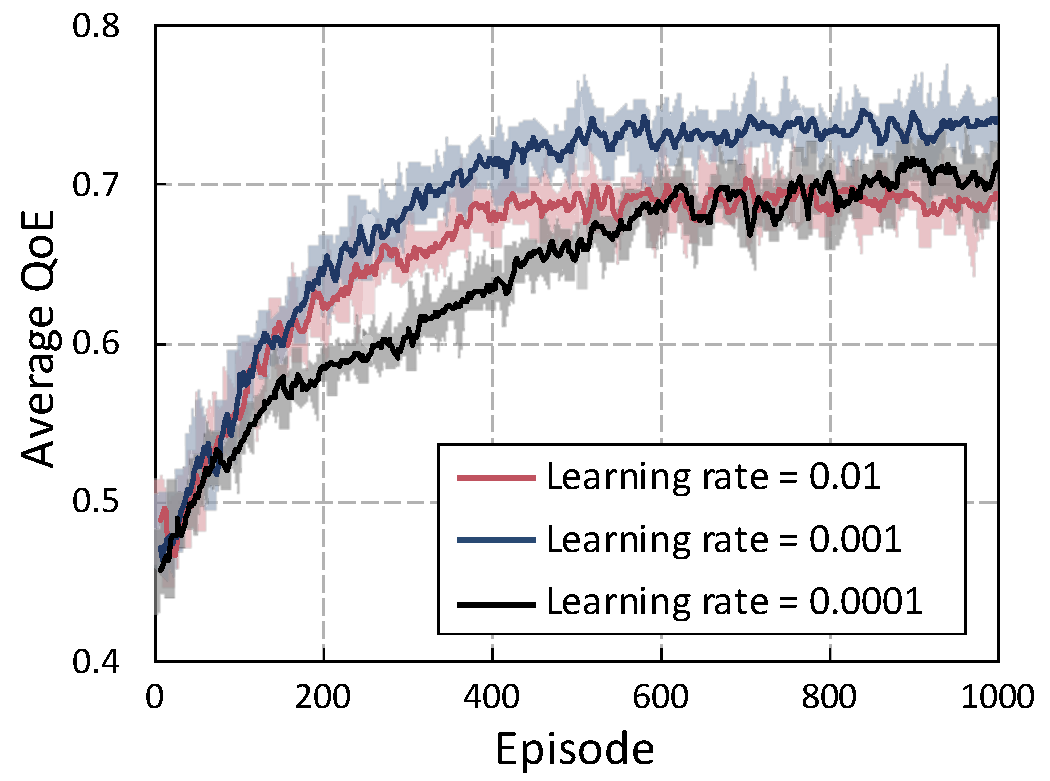
\includegraphics[width=\textwidth]{ conv1_f} 
		\textcolor{white}{i}\hspace{0.4cm}(a)
	\end{minipage}
	\hspace{-0.26cm}
	\begin{minipage}[b]{0.34\linewidth}
		\centering
		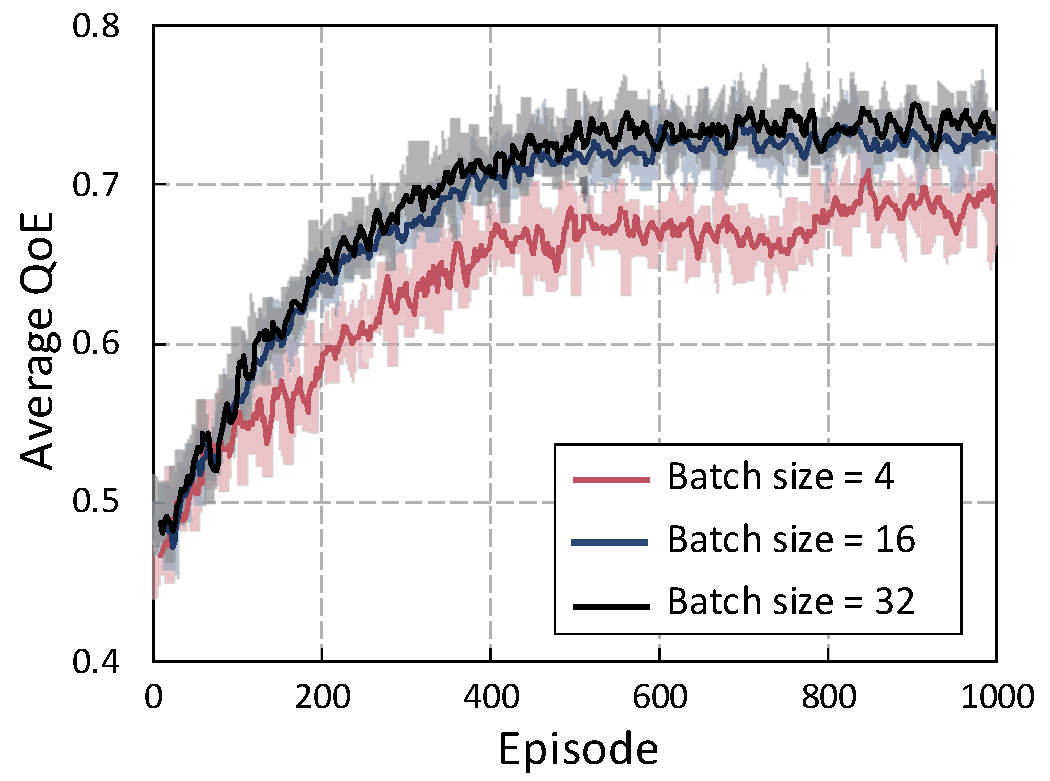
\includegraphics[width=\textwidth]{ conv2_f}
		\textcolor{white}{i}\hspace{0.4cm}(b)
	\end{minipage}

	\caption{The convergence of the average QoE across episodes under different hyper-parameters: (a) Learning rate; (b) Batch size.}
	\label{chart0}
\end{figure}




\section{Conclusion}\label{section:VI}
%In this study, our focus was directed towards addressing the challenge of offloading in MEC systems, where strict task processing deadlines and energy constraints adversely impact system performance. To address this challenge, we propose the QECO algorithm specifically designed to empower MDs to make offloading decisions without relying on knowledge about task models or other MDs' offloading decisions. The QECO algorithm not only adapts to the uncertain dynamics of load levels at ENs but also effectively manages the ever-changing system environment. Through extensive simulations, we demonstrate that QECO outperforms several established benchmark techniques. Specifically, it can significantly increase the average user's QoE. This advantage can lead to improvements in key performance metrics, including task completion rate, task delay, and energy consumption, according to the user's demands under different system conditions. 

%There are multiple directions for extend this research. A complementary approach involves extending the simplified task model by considering dependent divisible tasks that correspond to actual computational tasks. This can be achieved by incorporating a call graph~\cite{kwok1996dynamic} representation to develop relationships among task partitions. Furthermore, in order to accelerate the learning of optimal offloading policies, it is beneficial to enable MDs to take advantage of federated learning~\cite{li2020federated} techniques in the training process. This allows MDs to collectively contribute to improving the offloading model and enables continuous learning when new MDs join the network.

In this paper, we focused on addressing the challenge of offloading in MEC systems, where strict task processing deadlines and energy constraints adversely impact system performance. We formulated an optimization problem that aims to maximize the QoE of each MD individually, while QoE reflects the energy consumption and task completion delay. To address the dynamic and uncertain mobile environment, we proposed a QoE-oriented DRL-based computation offloading algorithm called QECO. Our proposed algorithm empowers MDs to make offloading decisions without relying on knowledge about task models or other MDs' offloading decisions. The QECO algorithm not only adapts to the uncertain dynamics of load levels at ENs, but also effectively manages the ever-changing system environment. Through extensive simulations, we showed that QECO outperforms several established benchmark techniques, while demonstrating a rapid training convergence. Specifically, QECO increases the average user's QoE by 37\% compared to an existing work. This advantage can lead to improvements in key performance metrics, including task completion rate, task delay, and energy consumption, under different system conditions and varying user demands.

There are multiple directions for future work. A complementary approach involves extending the task model by considering interdependencies among tasks. This can be achieved by incorporating a task call graph representation. Furthermore, in order to accelerate the learning of optimal offloading policies, it will be beneficial to take advantages of federated learning techniques in the training process. This will allow MDs to collectively contribute to improving the offloading model and enable continuous learning when new MDs join the network.



\newpage


\bibliographystyle{IEEEtran}
\bibliography{references}

\title{Responses to the Reviewers' Comments}

\maketitle

\vspace{-1.5cm}
\setstretch{1.6}

\setcounter{page}{1}

\begin{itemize}
	\item \textbf{Title of Manuscript}: A QoE-Oriented Computation Offloading Algorithm based on Deep Reinforcement Learning for Mobile Edge Computing
	
	
	\item \textbf{Authors}:  Iman Rahmati, Hamed Shah-Mansouri, and Ali Movaghar
	
	
	\item \textbf{Affiliation}: Departments of Electrical Engineering and Computer Engineering,  Sharif University of Technology, Tehran, Iran
	
	\item \textbf{Paper Reference Number}: TNSE-2024-03-0468 
	
\end{itemize}

\vspace{0.3cm}

\setstretch{1.2}

\noindent We would like to express our gratitude to the reviewers for their valuable recommendations toward improving the quality of our paper. We also want to gratefully thank the associate editor for handling the paper. Our responses to the reviewers' comments are given below. For convenience, we have used blue font for the revised or newly added paragraphs in the manuscript.\newline

\setcounter{section}{0}
\renewcommand*{\thesection}{\Roman{section}}
\makeatletter


\newpage

\section{Response to Reviewer 1}
\begin{enumerate}

\item \underline{Reviewer's Comment}: 
\textit{``(a) Lots of the studies focus on the research on resource optimisation of MEC by DRL, it is expected to survey the state-of-the-art within 3 years, and summarise it as an individual section, departing from the Section of Introduction. (b) Besides, the existing related work only has one paragraph without any discussion about the pros/cons of the previous work.''} \newline

\underline{Authors' Reply}: (a) To address the reviewer comment about state-of-the-art within 3 years discusion, we have added this paragraph to the Section I, as follows. \newline
	\begin{my}{1cm}{1cm}
	\rev{\,\,\,\, To cope with the dynamic nature of the network, recent research has proposed several task offloading algorithms using machine learning methods. In particular, reinforcement learning (RL) hold promises to determine optimal decision-making policies by capturing the dynamics of environments and learning strategies for accomplishing long-term objectives \cite{arulkumaran2017deep}. RL can effectively tackle the challenges of MEC arising from the ever-changing nature of networks, MDs, and servers' heterogeneity. This ultimately improves the MD users' QoE. We explore state-of-the-art RL-based techniques characteristic to discuss how they address task offloading problems in MEC. To minimize energy consumption, Munir \textit{et al.} \cite{munir2021multi} developed a semi-distributed approach using a multi-agent RL (MARL) framework for self-powered MEC. Gong \textit{et al.} in \cite{gong2022edge} proposed a DRL-based network structure in the industrial IoT (IIoT) systems to jointly optimize task offloading and resource allocation to achieve lower energy consumption and decreased task delay. To investigate privacy aware computation offloading problem, Wu \textit{et al.} in \cite{wu2024combining} proposed a deep Q-network (DQN)-based method. They transform the problem on MDP to optimize computation rate and energy consumption in a queuing-based IIoT network. Sun \textit{et al.} in \cite{sun2024hierarchical} explored both computation offloading and service caching problems in MEC. They formulated an optimization problem that aims to minimize the long-term average service delay. They then proposed a hierarchical DRL framework, which effectively handles both problems under heterogeneous resources.}
\end{my}


\vspace{6mm}

(b) We have also revised the ralated works section, as below.\\	 

	\begin{my}{1cm}{1cm}
	\rev{\,\,\,\, In recent years, edge computing has become a popular method for scenarios that need to process massive data with weak devices, such as IoTs \cite{zhang2023multi}, Internet of Vehicles (IoVs) \cite{lin2022multi}, \cite{wei2023many}, and Industrial IoT (IIoT) \cite{yuan2023adaptive} environment. To take advantage of RL methods for online computation offloading in MEC, Huang \textit{et al.} in \cite{huang2019deep}, focused on a wireless-powered MEC. They proposed a DRL-based approach, capable of attaining near-optimal decisions. This is achieved by selectively considering a compact subset of candidate actions in each iteration. Liu \textit{et al.} in \cite{liu2021learn} investigated a two-timescale computing offloading and resource allocation problem and proposed a resource coordination algorithm based on multi-agent DRL (MADRL), which can generate interactive information along with resource decisions. Zhou \textit{et al.} in \cite{zhou2021deep} used an MDP to model the interactions of the environment. They proposed a Q-learning approach to achieve optimal resource allocation strategies and computation offloading. Liao \textit{et al.} in \cite{liao2023online} introduced a double DRL algorithm for performing online computation offloading in MEC. This algorithm optimizes transmission power and scheduling of CPU frequency when minimizing both task computation delay and energy consumption.
		
	\,\,\,\, In these researches authors investigated simple MEC networks and explored computation offloading problems, mainly focused on delay-tolerant tasks or single MEC network model, and did not take into account the challenges of dynamic network environment with the variety of MDs and servers involved. In actual scenarios, an MEC system can provide delay-constrained services for serval MDs and ENs at the same time, while the works \cite{huang2019deep}, \cite{liu2021learn} not consider delay-sensitive tasks for network model and \cite{zhou2021deep}, \cite{liao2023online} just considered the situation of a single server or user in the MEC system.
	
\,\,\,\, In these researches authors investigated simple MEC networks and explored computation offloading problems, mainly focused on delay-tolerant tasks or single MEC network model, and did not take into account the challenges of dynamic network environment with the variety of MDs and servers involved. In actual scenarios, an MEC system can provide delay-constrained services for serval MDs and ENs at the same time, while the works \cite{huang2019deep}, \cite{liu2021learn} not consider delay-sensitive tasks for network model and \cite{zhou2021deep}, \cite{liao2023online} just considered the situation of a single server or user in the MEC system.

\,\,\,\, In fact, the state of MD's computing and transmission power, arrived task's requirement, the energy state of MDs, and workloads at ENs all change dynamically with time in actual systems, thus a more realistic MEC scenario is needed. Besides the works \cite{huang2019deep}--\cite{liao2023online}, Wu \textit{et al.} in \cite{wu2023computation} introduced a stochastic game-based resource allocation in the SDN-based MEC network. They used an MDP and proposed a MARL method to minimize both energy consumption and processing delay. Dai \textit{et al.} in \cite{dai2020edge} introduced the integration of action refinement into DRL and designed an algorithm to concurrently optimize resource allocation and computation offloading. To optimize privacy protection and quality of service, authors in \cite{wu2024privacy} investigated the joint computation offloading and power allocation problems for the IIoT network. They modeled the problem as an MDP and proposed a multi-agent DDQN-based algorithm.
In \cite{zhao2019deep}, Zhao \textit{et al.} proposed a computation offloading algorithm based on DRL, which addresses the competition for wireless channels to optimize long-term downlink utility. In this approach, each MD requires quality-of-service information from other MDs.


\,\,\,\, While studies like \cite{wu2023computation}--\cite{zhao2019deep} explored task offloading problems in a more advanced scenario and proposed some DRL-based algorithms, MEC systems often encounter challenges related to managing time-varying resource requests from heterogeneous devices, imposing significant challenges in resource accessibility and overall system performance. To address this issue, the authors applied queuing theory to model MEC systems more accurately, reflecting real-world scenarios. 
In \cite{Bolourian-WCL24}, the authors proposed an offloading algorithm using deep Q-learning for wireless-powered IoT devices in MEC systems. This algorithm aims to minimize the task drop rate while the devices solely rely on harvested energy for operation. Tang \textit{et al.} in \cite{9253665} investigated the task offloading problem for indivisible and deadline-constrained computational tasks in MEC systems. The authors proposed a distributed DRL-based offloading algorithm designed to handle uncertain workload dynamics at the ENs. 
In \cite{huang2021deadline}, Huang \textit{et al.} proposed a DRL-based method based on a partially observable MDP (POMDP), which guarantees the deadlines of real-time tasks while minimizing the total energy consumption of MDs. This algorithm effectively tackles the challenges of dynamic resource allocation in large-scale heterogeneous networks. To optimize delay and energy consumption in an MEC-based IIoT system, Wu \textit{et al.} in \cite{wu2023multi} proposed a multi-agent DQN-based method based on POMDP to address computation offloading problem. In \cite{gao2022large}, Gao \textit{et al.} introduced an attention-based multi-agent algorithm designed for decentralized computation offloading.}
\end{my}

\vspace{6mm}

We have also revised the motivation and contributions subsection, as below.

\vspace{6mm}

	\begin{my}{1cm}{1cm}
	\rev{\,\,\,\, Although DRL-based methods have demonstrated their effectiveness in handling network dynamics, task offloading still encounters several challenges that require further attention.  \textcolor{blue}{As shown in Table~\ref{table1}, current research primarily focuses on minimizing energy consumption \cite{tang2022uav}, reducing processing delays \cite{guo2022energy}, \cite{seo2022differential}, maximizing computation rates~\cite{huang2019deep}, or optimizing a weighted balance among performance factors \cite{li2022joint}. However, QoE is a time-varying performance measure that reflects user satisfaction and is not affected only by delay, as considered in \cite{sun2024hierarchical}, \cite{9253665} but also by energy consumption \cite{Bolourian-WCL24}, \cite{huang2021deadline}. A more comprehensive approach is required to address the dynamic requirements of individual users in real-time scenarios with multiple MDs and ENs. 
    While some existing works such as \cite{liao2023online}, \cite{wu2024privacy}, \cite{dai2020edge}, \cite{gao2022large}, \cite{li2022joint} have investigated the trade-off between delay and energy consumption, they fail to address the user demands and fulfill QoE requirements properly.} In contrast to the aforementioned works, we propose a DRL-based distributed algorithm that provides users with an appropriate balance among QoE factors based on their demands.}
\end{my}



\newpage

\item \underline{Reviewer's Comment}: 
\textit{``Please highlight what and how the proposed approach provides "high performance" to further specify the motivations and contributions. Especially, please highlight the reason why the authors design the framework by integrating LSTM. Otherwise, it will make the innovations seem weak.''} \newline





\underline{Authors' Reply}:\\

\item \underline{Reviewer's Comment}: 
\textit{``In section III, why is the size of the task selected from a discrete set? Is it selected randomly or in another way? Besides, the authors define the offloading indicate function as $y_{i,j}(t)$, it should be involved when modelling the Edge Execution phrase.''} \newline

\underline{Authors' Reply}:\\

\item \underline{Reviewer's Comment}: 
\textit{``Some sota methods (e.g., DDQN, DDPG) are expected to be compared in the section on performance evaluation, and authors should have more discussions about the evaluation results rather than merely introducing them. \textcolor{red}{Besides, I think it is better to design the evaluations with a real dataset. Besides, 9\% and 6\% are not significant improvements compared to other methods.''}} \newline

\underline{Authors' Reply}:\\

\item \underline{Reviewer's Comment}: 
\textit{``Other concerns are also expected to be addressed: (a) be careful to use words like "battery level" to express the energy consumption, because some of the energy is provided by the wired line power. (b) Most of the references are out of 3 years, please investigate more studies published in recent years. (c) \textcolor{red}{The authors should thoroughly check the writing style, grammar, and spelling to enhance the paper's clarity, conciseness, and overall impact.}}''\newline

\underline{Authors' Reply}: (a) We have changed the word "battery level" to "energy state" in whole paper of the revised manuscript. \newline

(b) We have added some related refrences, which are under 3 years, in Section I, as follow: \newline

		\begin{my}{1cm}{1cm}
	\rev{
		{\small
			\noindent\hspace{-0.3mm}\cite{munir2021multi} Munir, Md Shirajum and Tran, Nguyen H and Saad, Walid and Hong, Choong Seon, ``Multi-agent meta-reinforcement learning for self-powered and sustainable edge computing systems,'' \textit{IEEE Trans. Netw. Serv. Manag.}, vol. 18, no. 3, pp. 3353-3374. 2021.\\[6pt]
			\cite{wu2024combining} G. Wu, X. Chen, Y. Shen, Z. Xu, H. Zhang, S. Shen, and S. Yu,``Combining Lyapunov optimization with Actor-Critic networks for privacy-aware IIoT computation offloading,'' in \textit{IEEE Internet Things J.}, 2024, Early Access\\[6pt]
			\cite{lin2022multi} Lin, Shih-Yang and Huang, Chung-Ming and Wu, Tzu-Yu, ``Multi-access edge computing-based vehicle-vehicle-RSU data offloading over the multi-RSU-overlapped environment,'' \textit{IEEE Open J. Intell. Transp. Syst.}, vol. 3, pp. 7--32, 2022.\\[6pt]
			\cite{wei2023many} Wei, Zhiwei and Li, Bing and Zhang, Rongqing and Cheng, Xiang and Yang, Liuqing, ``Many-to-many task offloading in vehicular fog computing: A multi-agent deep reinforcement learning approach,'' \textit{IEEE Trans. Mob. Comput.}, vol. 23, no. 3, pp. 2107--2122, 2023.\\[6pt]
			\cite{wu2023multi} G. Wu, Z. Xu, H. Zhang, S. Shen, and S. Yu,  ``Multi-agent DRL for joint completion delay and energy consumption with queuing theory in MEC-based IIoT,'' in \textit{Journal of Parallel and Distributed Computing}, vol. 176, pp. 80–94, Jun. 2023.\\[6pt]
			\cite{wu2023computation} G. Wu, H. Wang, H. Zhang, Y. Zhao, S. Yu, and S. Shen, ``Computation offloading method using stochastic games for software-defined-network-based multiagent mobile edge computing,'' \textit{IEEE Internet Things J.}, vol. 10, no. 20, pp. 17620–17634, Oct. 2023.\\[6pt]
			\cite{wu2024privacy} G. Wu, X. Chen, Z. Gao, H. Zhang, S. Yu, and S. Shen, ``Privacy-preserving offloading scheme in multi-access mobile edge computing based on MADRL,'' \textit{Journal of Parallel and Distributed Computing}, vol. 10, no. 1, pp. 451--460, Mar. 2022.\\[6pt]
			\cite{yuan2023adaptive} Yuan, Shijing and Dong, Beiyu and Lvy, Hongtao and Liu, Hongze and Chen, Hongyang and Wu, Chentao and Guo, Song and Ding, Yue and Li, Jie, ``Adaptive incentivize for cross-silo federated learning in IIoT: A multi-agent reinforcement learning approach,'' \textit{IEEE Internet Things J.}, 2023.\\[6pt]
			\cite{zhang2023multi} Zhang, Jing and Shen, Fei and Tang, Liang and Yan, Feng and Qin, Fei and Wang, Chao, ``A Multi-Agent Reinforcement Learning Approach for Dynamic Offloading with Partial Information-Sharing in IoT Networks,'' \textit{2023 IEEE 98th Vehicular Technology Conference (VTC2023-Fall)}, pp. 1--5, 2023.\\[6pt]
			\cite{tang2022uav} Tang, Qiang and Liu, Lixin and Jin, Caiyan and Wang, Jin and Liao, Zhuofan and Luo, Yuansheng, ``An UAV-assisted mobile edge computing offloading strategy for minimizing energy consumption,'' \textit{Computer Networks}, vol. 207, pp. 108857, 2022.\\[6pt]
			\cite{seo2022differential} Seo, Hyeonseok and Oh, Hyeontaek and Choi, Jun Kyun and Park, Sangdon, ``Differential pricing-based task offloading for delay-sensitive IoT applications in mobile edge computing system,'' \textit{IEEE Internet Things J.}, vol. 9, no. 19, pp. 19116--19131, 2022.\\[6pt]
			\cite{guo2022energy} Guo, Mian and Li, Qirui and Peng, Zhiping and Liu, Xiushan and Cui, Delong, ``Energy harvesting computation offloading game towards minimizing delay for mobile edge computing,'' \textit{Computer Networks}, vol. 204, pp. 108678, 2022.\\[6pt]
			\cite{li2022joint} Li, Yuwei and Yang, Bo and Wu, Hao and Han, Qiaoni and Chen, Cailian and Guan, Xinping, ``Joint offloading decision and resource allocation for vehicular fog-edge computing networks: A contract-stackelberg approach,'' \textit{IEEE Internet Things J.}, vol. 9, no. 17, pp. 15969--15982, 2022.\\[10pt]}\\}
\end{my}

(c)


\end{enumerate}


\newpage

\section{Response to Reviewer 2}
\begin{enumerate}
	
	\item \underline{Reviewer's Comment}: 
	\textit{``The authors should provide a comparative table to highlight their contributions. Specially, the authors should compare their method with other references on computation task offloading cited in the paper, including aspects such as scenarios, methods, advances, drawbacks, and so on.''} \newline

	\underline{Authors' Reply}: To address the reviewer's comment, we have included a table in the 'Related Works' subsection that compares the key characteristics of relevant studies, as below:
	\begin{table*}[htbp]\textcolor{blue}{
			\renewcommand{\arraystretch}{0.6}
			\captionsetup{name=TABLE}
			\caption{\textcolor{blue}{Comparison of Related Works Characteristic\vspace{4mm}}}
			\scalebox{0.7}{%
				\begin{tabular}{ lp{3.4cm}p{4.5cm}p{5.2cm}p{1.7cm}p{3cm}p{4.6cm}l} 
					\toprule
					\textbf{Paper} & \textbf{Scenario} &  \textbf{Problem} &  \textbf{Objective} &  \textbf{Model} & \textbf{Method} &  \textbf{Drawbacks}  \\ \midrule
					\cite{liao2023online} & Queuing-based MEC & Online computation offloading & Minimize computation delay and energy consumption & MDP & DDQN & Only for a singel MEC system model  \\\midrule
					\cite{zhou2021deep} & heterogeneous MEC & Resource allocation and computation offloading & Minimize energy consumption of the entire system & MDP & DDQN & Only for a singel MEC system model \\\midrule				
					\cite{huang2019deep} & Wireless-powered MEC & Computation offloading and resource allocations & Maximize computation rate & MIP & DQN & Not consider delay-sensitive tasks \\\midrule
					\cite{wu2024privacy} & MEC-based IIoT  & Joint power allocation and computation offloading  & Optimization of privacy protection and quality of service. & MDP & Multi-agent DDPG & Not take user's deman into consideration \\\midrule
					\cite{zhao2019deep} & MEC & User association and resource allocation & Optimize downlink utility & MDP & Multi-agent D3QN & Not consider system delay and energy consumtion \\\midrule
					\cite{sun2024hierarchical} & MEC & Computation offloading and service caching & Minimize average service delay & MDP & hierarchical DRL & Not consider system energy consumtion \\\midrule
					\cite{wu2023computation} & SDN-based MEC & Stochastic game-based resource allocation & Minimize energy consumption and processing delay & MDP & MARL & Not consider tasks with maximum delay tolerance\\\midrule
					\cite{dai2020edge} & MEC & Resource allocation and computation offloading & Minimize energy consumption & MDP & DDPG & Not take user's deman into consideration \\\midrule
					\cite{liu2021learn} & MEC & Resource allocation and computation offloading & Minimize execution cost & POMDP & MADRL &  Not consider delay-sensitive tasks \\\midrule
					\cite{gong2022edge} & MEC-based IIoT & Resource allocation and computation offloading & Minimize task computation delay and energy consumption & MDP & DRL & Not take user's deman into consideration\\\midrule
					\cite{gao2022large} & Queuing-based heterogeneous MEC & Decentralized computation offloading & Optimize system cost and completion rates & MDP & Multi-agent DDPG & Not take user's deman into consideration \\\midrule
					\cite{9253665} &  Queuing-based MEC &  Computation offloading & Minimize drop rate and computation delay. & MDP & D3QN + LSTM & Not consider system energy consumtion\\\midrule
					\cite{wu2024combining} & Queuing-based IIoT MEC & Privacy aware computation offloading & Optimization of computation rate and energy consumption & MDP & DDPG  & Not take user's deman into consideration \\\midrule
					\cite{wu2023multi} & Queuing-based IIoT MEC & Computation offloading & Optimize delay and energy consumption & POMDP & Multi-agent DQN&  Not consider tasks with maximum delay tolerance \\\midrule
					\cite{huang2021deadline} & Queuing-based MEC & Computation offloading & Optimize drop rate and energy consumption & POMDP & DDPG & Not consider computation delay \\ \midrule
					\cite{Bolourian-WCL24} & Queuing-based MEC with EHs& Energy harvesting  computation offloading & Minimize drop rate and energy consumption. & MDP  & DQN & Not consider computation delay  \\\midrule
					QECO &  Queuing-based MEC &  Computation offloading & Maximize the QoE of each MD individually &MDP & D3QN + LSTM & \\
					\toprule
			\end{tabular}}
			\label{table1}}
	\end{table*}
	\item \underline{Reviewer's Comment}: 
	\textit{``I think more explanations should be added for the QoE function. How can the defined function reflect QoE?''} \newline
	
	\underline{Authors' Reply}: 

	\item \underline{Reviewer's Comment}: 
	\textit{``(a) What inputs and outputs of Algorithm 2? (b) They should be added to make readers clearly understand the results.''} \\\newline
	\underline{Authors' Reply}: (a) To address the reviewer concern about algorithm 2, we have revised secound paragraph of subsection (Training Process Algorithm at EN $j \in \mathcal{J})$ in Section IV to clarify the inputs and outputs of algorithms 2, as follows. \newline
	
	\begin{my}{1cm}{1cm}
		\rev{In particular, regarding experience $n$, the target-Q value $\hat{Q}_{i,n}^{\text{T}}$ represents the long-term QoE for action $\boldsymbol{a}_i(n)$ under state $\boldsymbol{s}_i(n)$. This value corresponds to the QoE observed in experience $n$, as well as the approximate expected upcoming QoE. 
			\textcolor{blue}{Based on the previous sample experiences $\mathcal{N}$, the EN computes the vector $\hat{\mathbf{Q}}_i^{\text{T}} = (\hat{Q}^{\text{T}}_{i,n})_{n \in \mathcal{N}}$ and trains the MD's neural network (in steps 11-21 of Algorithm ~\ref{alg:cap2}) to keep parameter vector $\theta^{\text{E}}_i$ in $\textit{Net}_i^{\text{E}}$ update for the MD's \textit{UpdateRequest}}. The key idea of updating $\textit{Net}_i^{\text{E}}$ is to minimize the disparity in Q-values between $\textit{Net}_i^{\text{E}}$ and $\textit{Net}_i^{\text{T}}$, as indicated by the following loss function:\\ \dots}
	\end{my}
		
	We have also revised algorithm 1 and 2, as below.\\	
	

\begin{my}{0.5cm}{0.5cm}	
\rev{\begin{minipage}[b]{0.87\textwidth} 
	\begin{algorithm}[H] \caption{QECO Algorithm (Training Process)}\label{alg:cap2} \centering 
		\begin{algorithmic}[1] \renewcommand{\algorithmicrequire}{\textbf{\textcolor{blue}{Input:}}} \renewcommand{\algorithmicensure}{\textbf{\textcolor{blue}{Output:}}} \Require \textcolor{blue}{experience $(\boldsymbol{s}_i(t), \boldsymbol{a}_i(t), \boldsymbol{q}_i(t), \boldsymbol{s}_i(t+1))$ from MD $i \in \mathcal{I}$} \Ensure \textcolor{blue}{parameter vector $\theta_i^{\text{E}}$} 
	\end{algorithmic} 
\end{algorithm} 
\end{minipage}
\vspace{5mm}

\begin{minipage}[b]{0.87\textwidth} 
	\begin{algorithm}[H] \caption{QECO Algorithm (Offloading Decision)}\label{alg:cap2} \centering 
		\begin{algorithmic}[1] \renewcommand{\algorithmicrequire}{\textbf{Input:}} \renewcommand{\algorithmicensure}{\textbf{Output:}}\Require state space $\mathcal{S}$, action space $\mathcal{A}$
			\Ensure MD $i \in \mathcal{I}$ experience  \textcolor{blue}{ $(\hspace{-0.2mm}\boldsymbol{s}_i(\hspace{-0.2mm}t\hspace{-0.2mm}), \boldsymbol{a}_i(\hspace{-0.2mm}t\hspace{-0.2mm}), \boldsymbol{q}_i(\hspace{-0.2mm}t\hspace{-0.2mm}), \boldsymbol{s}_i(\hspace{-0.2mm}t\hspace{-0.3mm}+\hspace{-0.3mm}\hspace{-0.2mm}1\hspace{-0.2mm}\hspace{-0.2mm})\hspace{-0.2mm})$}
		\end{algorithmic} 
	\end{algorithm} 
\end{minipage}}
\end{my}
	

\vspace{10mm}
	\item \underline{Reviewer's Comment}: 
	\textit{``The authors should open their experiments in github, so that other researchers can compare their work with other ones.''} \newline
	\underline{Authors' Reply}: To address the reviewer comment, we make our experiments more accessible by sharing our GitHub rerepository. We have added it into the end of first paragraph of Section V, as follows.
	\begin{my}{1cm}{1cm}
		\rev{Detailed settings regarding the neural networks and simulation can be found at our github repository. }
	\end{my}
	We have also provided repository URL link in the footnote of Page 8 as below.
	\begin{my}{1cm}{1cm}
		\rev{The code for reproducing the simulation results of this letter is available at\newline https://github.com/ImanRHT/QECO.} \newline
	\end{my}

\newpage

	\item \underline{Reviewer's Comment}: 
	\textit{``The following references closely related to the current work should be discussed or compared with the current work for completeness.''} \newline
		\begin{my}{1cm}{1cm}
		\rev{
			{\small
				\noindent\hspace{-0.5mm}\cite{wu2024combining}  G. Wu, X. Chen, Y. Shen, Z. Xu, H. Zhang, S. Shen, and S. Yu,``Combining Lyapunov optimization with Actor-Critic networks for privacy-aware IIoT computation offloading,'' in \textit{IEEE Internet of Things Journal}, 2024, Early Access\\[6pt]
				\cite{wu2023computation} G. Wu, H. Wang, H. Zhang, Y. Zhao, S. Yu, and S. Shen, ``Computation offloading method using stochastic games for software-defined-network-based multiagent mobile edge computing,'' \textit{IEEE Internet of Things Journal}, vol. 10, no. 20, pp. 17620–17634, Oct. 2023.\\[6pt]
				\cite{wu2024privacy} G. Wu, X. Chen, Z. Gao, H. Zhang, S. Yu, and S. Shen, ``Privacy-preserving offloading scheme in multi-access mobile edge computing based on MADRL,'' \textit{Journal of Parallel and Distributed Computing}, vol. 10, no. 1, pp. 451--460, Mar. 2022.\\[6pt]
				\cite{wu2023multi} G. Wu, Z. Xu, H. Zhang, S. Shen, and S. Yu,  ``Multi-agent DRL for joint completion delay and energy consumption with queuing theory in MEC-based IIoT,'' in \textit{Journal of Parallel and Distributed Computing}, vol. 176, pp. 80–94, Jun. 2023\\[10pt]}\\}
	\end{my}

	
	\underline{Authors' Reply}:\\
	
	We have cited these works in the Section I of the revised manuscript.\\


	
\end{enumerate}

\vfill

We would like to gratefully thank the reviewer for the valuable comments and suggestions. We hope that we have satisfactorily addressed these comments.\newline

\end{document}


